
% ----------------------------------------------------------------------
%                   LATEX TEMPLATE FOR PhD THESIS
% ----------------------------------------------------------------------

% based on Harish Bhanderi's PhD/MPhil template, then Uni Cambridge
% http://www-h.eng.cam.ac.uk/help/tpl/textprocessing/ThesisStyle/
% corrected and extended in 2007 by Jakob Suckale, then MPI-CBG PhD programme
% and made available through OpenWetWare.org - the free biology wiki


%: Style file for Latex
% Most style definitions are in the external file PhDthesisPSnPDF.
% In this template package, it can be found in ./Latex/Classes/
\documentclass[twoside,11pt]{Latex/Classes/PhDthesisPSnPDF}

%: Macro file for Latex
% Macros help you summarise frequently repeated Latex commands.
% Here, they are placed in an external file /Latex/Macros/MacroFile1.tex
% An macro that you may use frequently is the figuremacro (see introduction.tex)
% This file contains macros that can be called up from connected TeX files
% It helps to summarise repeated code, e.g. figure insertion (see below).

\hyphenation{Myspace}
\hyphenation{Facebook}
\hyphenation{DBpedia}
\hyphenation{eSpeak}

\newenvironment{small_itemize}{
\begin{itemize}
  \setlength{\itemsep}{1pt}
  \setlength{\parskip}{0pt}
  \setlength{\parsep}{0pt}
}{\end{itemize}}

% \usepackage{chapterbib}
\usepackage{slashbox}
\usepackage{nomencl}
\makenomenclature

\usepackage{eurosym}
\usepackage{pbox}
\usepackage{fancybox}
\usepackage{amsmath}
\usepackage{enumitem}

\usepackage{rotating}

\newcommand{\superscript}[1]{\ensuremath{^{\textrm{#1}}}}
\newcommand{\subscript}[1]{\ensuremath{_{\textrm{#1}}}}

% thumbnail environment
\newcommand{\eventtitle}[1]{{\hbox{\strut \textbf{#1}}}}
\newcommand{\thumbheight}{14mm}
\newcommand{\newstrip}{\newline\vspace{-1em}\newline}
\newenvironment{thumbsequence}{}{\makebox[1mm]{}}

% linewrap symbol
\usepackage{MnSymbol}
\definecolor{grey}{RGB}{160,160,160}
\newcommand{\linewrap}{\raisebox{-.4ex}{\textcolor{grey}{$\rhookleftarrow$}}}

% todo macro
\usepackage{color}
\newcommand{\todo}[1]{\noindent\textcolor{red}{{\bf \{TODO}: #1{\bf \}}}}

\usepackage{xspace}
\DeclareRobustCommand{\googleplus}{\mbox{Google\hspace{0em}\raisebox{.28ex}{\tiny\bf +}\kern-0.2ex}\xspace}
\newcommand{\gplus}{\mbox{G\hspace{0em}\raisebox{.28ex}{\tiny\bf +}\kern-0.2ex}\xspace}
\newcommand{\plusone}{\mbox{\hspace{0em}\raisebox{.28ex}{\tiny\bf +}\kern-0.2ex 1}\xspace}

% insert a centered figure with caption and description
% parameters 1:filename, 2:title, 3:description and label
\newcommand{\figuremacro}[3]{
	\begin{figure}[!ht]
		\centering
		\includegraphics[width=1\textwidth]{#1}
		\caption[#2]{\textbf{#2} - #3}
		\label{fig:#1}
	\end{figure}
}

% insert a centered figure with caption and description AND WIDTH
% parameters 1:filename, 2:title, 3:description and label, 4: textwidth
% textwidth 1 means as text, 0.5 means half the width of the text
\newcommand{\figuremacroW}[4]{
	\begin{figure}[!ht]
		\centering
		\includegraphics[width=#4\textwidth]{#1}
		\caption[#2]{\textbf{#2} - #3}
		\label{fig:#1}
	\end{figure}
}

% inserts a figure with wrapped around text; only suitable for NARROW figs
% o is for outside on a double paged document; others: l, r, i(inside)
% text and figure will each be half of the document width
% note: long captions often crash with adjacent content; take care
% in general: above 2 macro produce more reliable layout
\newcommand{\figuremacroN}[3]{
	\begin{wrapfigure}{o}{0.5\textwidth}
		\centering
		\includegraphics[width=0.48\textwidth]{#1}
		\caption[#2]{{\small\textbf{#2} - #3}}
		\label{fig:#1}
	\end{wrapfigure}
}

% predefined commands by Harish
\newcommand{\PdfPsText}[2]{
  \ifpdf
     #1
  \else
     #2
  \fi
}

\newcommand{\IncludeGraphicsH}[3]{
  \PdfPsText{\includegraphics[height=#2]{#1}}{\includegraphics[bb = #3, height=#2]{#1}}
}

\newcommand{\IncludeGraphicsW}[3]{
  \PdfPsText{\includegraphics[width=#2]{#1}}{\includegraphics[bb = #3, width=#2]{#1}}
}

\newcommand{\InsertFig}[3]{
  \begin{figure}[!ht]
    \begin{center}
      \leavevmode
      #1
      \caption{#2}
      \label{#3}
    \end{center}
  \end{figure}
}


%%% Local Variables: 
%%% mode: latex
%%% TeX-master: "~/Documents/LaTeX/CUEDThesisPSnPDF/thesis"
%%% End: 




%: ----------------------------------------------------------------------
%:                  TITLE PAGE: name, degree,..
% ----------------------------------------------------------------------
% below is to generate the title page with crest and author name

%if output to PDF then put the following in PDF header
\ifpdf  
    \pdfinfo { /Title  (PhD and MPhil Thesis Classes)
               /Creator (TeX)
               /Producer (pdfTeX)
               /Author (YourName your@email.net)
               /CreationDate (D:YYYYMMDDhhmmss)  %format D:YYYYMMDDhhmmss
               /ModDate (D:YYYYMMDDhhmm)
               /Subject (xyz)
               /Keywords (add, your, keywords, here) }
    \pdfcatalog { /PageMode (/UseOutlines)
                  /OpenAction (fitbh)  }
\fi


\title{Enriching Unstructured Media Content About Events to Enable Semi-Automated Summaries, Compilations, and Improved Search by Leveraging Social Networks}



% ----------------------------------------------------------------------
% The section below defines www links/email for author and institutions
% They will appear on the title page of the PDF and can be clicked
\ifpdf
  \author{\href{mailto:tsteiner@lsi.upc.edu}{Thomas Steiner}}
%  \cityofbirth{born in XYZ} % uncomment this if your university requires this
%  % If city of birth is required, also uncomment 2 sections in PhDthesisPSnPDF
%  % Just search for the "city" and you'll find them.
  \collegeordept{\href{http://www.lsi.upc.edu/}{Departament de Llenguatges i Sistemes Informàtics}}
  \university{\href{http://www.upc.edu/}{Universitat Politècnica de Catalunya}}

  % The crest is a graphics file of the logo of your research institution.
  % Place it in ./frontmatter/figures and specify the width
  \crest{\includegraphics[width=4cm]{upc-logo}}
  
% If you are not creating a PDF then use the following. The default is PDF.
\else
  \author{Thomas Steiner}
%  \cityofbirth{born in XYZ}
  \collegeordept{Departament de Llenguatges i Sistemes Informàtics}
  \university{Universitat Politècnica de Catalunya}
  \crest{\includegraphics[width=4cm]{logo}}
\fi

%\renewcommand{\submittedtext}{change the default text here if needed}
\degree{Philosophi{\ae} Doctor (PhD)}
\degreedate{December 2012}


% ----------------------------------------------------------------------
       
% turn of those nasty overfull and underfull hboxes
\hbadness=10000
\hfuzz=50pt


%: --------------------------------------------------------------
%:                  FRONT MATTER: dedications, abstract,..
% --------------------------------------------------------------

\begin{document}

%\language{english}

% sets line spacing
\renewcommand\baselinestretch{1.2}
\baselineskip=18pt plus1pt


%: ----------------------- generate cover page ------------------------

\maketitle  % command to print the title page with above variables


%: ----------------------- cover page back side ------------------------
% Your research institution may require reviewer names, etc.
% This cover back side is required by Dresden Med Fac; uncomment if needed.

\newpage
\vspace{10mm}
1$^{st}$ Advisor: Joaquim Gabarró Vallés (UPC)

\vspace{10mm}
2$^{nd}$ Advisor: Michael Hausenblas (DERI)

\vspace{20mm}
Day of the defense: \todo{add date of the defense}

\vspace{20mm}
\hspace{70mm}Signature from head of PhD committee:



%: ----------------------- abstract ------------------------

% Your institution may have specific regulations if you need an abstract and where it is to be placed in the document. The default here is just after title.


% Thesis Abstract -----------------------------------------------------


%\begin{abstractslong}    %uncommenting this line, gives a different abstract heading
\begin{abstracts}        %this creates the heading for the abstract page
Mobile devices like smartphones and digital cameras together with social networks enable people to generate,
share, and consume enormous amounts of media items, both \textit{en route} or at home.
Common search operations, for example searching for a single music video based on artist
and title on video platforms such as YouTube,
can be achieved both based on potentially shallow human-generated metadata,
or based on more profound content analysis,
driven by Optical Character Recognition (OCR) or Automatic Speech Recognition (ASR).
However, more advanced use cases, such as \emph{summaries} or \emph{compilations} of \emph{several} media items
covering a certain event, are hard, if not impossible to fulfill at large scale.
Example events can be a keynote speech at a conference,
a music concert in a stadium, or a natural catastrophe in a country.
At such events, given a stable network connection,
media items are published on social networks as the event happens.
The main research question can thus be formulated as\\

\noindent \textit{``Can user-customizable media galleries that summarize given events
be\linebreak created solely based on textual and multimedia data from social networks?''}\\

In this thesis, we develop a novel interactive Web application for media item enrichment,
leveraging social networks, utilizing the Web of Data,
Content-based Image and Video Retrieval (CBIR, CBVR) techniques,
and fine-grained media item addressing schemes like Media Fragments URIs,
to provide a scalable and near realtime solution to realize the above use cases.
We detail and evaluate our approach:
first, we recognize and disambiguate named entities in relevant microposts
from social networks that contain links to media items, or to pages that host media items.
Second, we extract the raw media item data from social networks and relate them to the originating micropost.
Third, we deduplicate media items using CBIR and CBVR techniques.
Fourth, we rank the deduplicated list of media items according to specified ranking criteria,
and finally compile the top-$n$ ranked media items to a user-customizable media gallery.

\end{abstracts}
%\end{abstractlongs}

% ---------------------------------------------------------------------- 


% The original template provides and abstractseparate environment, if your institution requires them to be separate. I think it's easier to print the abstract from the complete thesis by restricting printing to the relevant page.
% \begin{abstractseparate}
%   
% Thesis Abstract -----------------------------------------------------


%\begin{abstractslong}    %uncommenting this line, gives a different abstract heading
\begin{abstracts}        %this creates the heading for the abstract page
Mobile devices like smartphones and digital cameras together with social networks enable people to generate,
share, and consume enormous amounts of media items, both \textit{en route} or at home.
Common search operations, for example searching for a single music video based on artist
and title on video platforms such as YouTube,
can be achieved both based on potentially shallow human-generated metadata,
or based on more profound content analysis,
driven by Optical Character Recognition (OCR) or Automatic Speech Recognition (ASR).
However, more advanced use cases, such as \emph{summaries} or \emph{compilations} of \emph{several} media items
covering a certain event, are hard, if not impossible to fulfill at large scale.
Example events can be a keynote speech at a conference,
a music concert in a stadium, or a natural catastrophe in a country.
At such events, given a stable network connection,
media items are published on social networks as the event happens.
The main research question can thus be formulated as\\

\noindent \textit{``Can user-customizable media galleries that summarize given events
be\linebreak created solely based on textual and multimedia data from social networks?''}\\

In this thesis, we develop a novel interactive Web application for media item enrichment,
leveraging social networks, utilizing the Web of Data,
Content-based Image and Video Retrieval (CBIR, CBVR) techniques,
and fine-grained media item addressing schemes like Media Fragments URIs,
to provide a scalable and near realtime solution to realize the above use cases.
We detail and evaluate our approach:
first, we recognize and disambiguate named entities in relevant microposts
from social networks that contain links to media items, or to pages that host media items.
Second, we extract the raw media item data from social networks and relate them to the originating micropost.
Third, we deduplicate media items using CBIR and CBVR techniques.
Fourth, we rank the deduplicated list of media items according to specified ranking criteria,
and finally compile the top-$n$ ranked media items to a user-customizable media gallery.

\end{abstracts}
%\end{abstractlongs}

% ---------------------------------------------------------------------- 

% \end{abstractseparate}


%: ----------------------- tie in front matter ------------------------

\frontmatter
% Thesis Dedictation ---------------------------------------------------

\begin{dedication} %this creates the heading for the dedication page
\todo{write dedication}
\end{dedication}

% ----------------------------------------------------------------------
\begin{acknowledgements}

\textbf{Personal Acknowledgements:}

First and foremost, I~would like to thank my wife Laura
for her support, understanding, patience, and energy
during my time as a~PhD student, and simply for being at my side.
Without you, I~would not be where I~am today.

I~wholeheartedly thank my two advisors Joaquim Gabarró Vallés
and Michael Hausenblas for their guidance, helpful comments,
informative pointers, and especially
for their constructive criticisms.
The areas of research that I~have tackled in this thesis
are still young and sometimes uncharted territory.
I~am very thankful that the two of you have ventured
on the undertaking of leading me through this thesis.

I~deeply appreciate all the review comments, thoughts, challenging questions,
and, last not least, the \LaTeX~help of my dear friend
and research colleague Ruben Verborgh.
It was, is, and will be an honor to work with you.
My warm thanks also go to Raphaël Troncy and his team
at \mbox{EURECOM} Sophia Antipolis in France
who have helped shape some of the ideas presented in this thesis.

I~would like to thank my former and current managers at Google,
namely N.~Kryvossidis, R.~Ashley, C.~Bouchère, and I.~Sassarini
for their support for my thesis.
A~lot of valuable input for my thesis came in via social networks.
My thanks go out to everyone I have interacted with
around the hashtag \texttt{\#TomsPhD}
on Twitter, \googleplus, and Facebook.

Finally, I~sincerely thank my parents and my brother
who have made me the person I~am today.
My parents have taught me
not to go for the easy choices, even
if at times they may seem tempting,
but instead to try harder and never give up.
This thesis also is for you.

\textbf{Formal Acknowledgements:}

The research presented in this doctoral thesis
was partially supported by the European Commission
under Grant No.~248296 with the European Union (FP7~ICT~STReP)
project \mbox{\emph{I-SEARCH}}.

\vspace{80mm}

\textbf{To cite this document:}

\small
\begin{verbatim}
  @phdthesis{steiner2013thesis,
    author = {Thomas Steiner},
    title  = {Enriching Unstructured Media Content About Events to
              Enable Semi-Automated Summaries, Compilations, and
              Improved Search by Leveraging Social Networks},
    year   = {2013},
    school = {Universitat Polit\`{e}cnica de Catalunya}
  }
\end{verbatim}

\normalsize

\vspace{10mm}
\textbf{Copyright and License:}\\\\
\small \copyright \normalsize 2013 Thomas Steiner\\
Licensed under the Creative Commons Attribution-ShareAlike 3.0 License.\\
\url{http://creativecommons.org/licenses/by-sa/3.0/}

\end{acknowledgements}



%: ----------------------- contents ------------------------

\setcounter{secnumdepth}{3} % organisational level that receives a numbers
\setcounter{tocdepth}{3}    % print table of contents for level 3
\tableofcontents            % print the table of contents
% levels are: 0 - chapter, 1 - section, 2 - subsection, 3 - subsection


%: ----------------------- list of figures/tables ------------------------

\listoffigures	% print list of figures

\listoftables  % print list of tables


%: ----------------------- glossary ------------------------

% Tie in external source file for definitions: /frontmatter/glossary.tex
% Glossary entries can also be defined in the main text. See glossary.tex
% this file is called up by thesis.tex
% content in this file will be fed into the main document

% Glossary entries are defined with the command \nomenclature{1}{2}
% 1 = Entry name, e.g. abbreviation; 2 = Explanation
% You can place all explanations in this separate file or declare them in the middle of the text. Either way they will be collected in the glossary.

% required to print nomenclature name to page header
\markboth{\MakeUppercase{\nomname}}{\MakeUppercase{\nomname}}

\nomenclature{NLP}{Natural Language Processing}
\nomenclature{CBIR}{Content-based Image Retrieval} 
\nomenclature{CBVR}{Content-based Video Retrieval} 
\nomenclature{RDF}{Resource Description Framework}
\nomenclature{W3}{World-Wide Web}
\nomenclature{WWW}{World-Wide Web}
\nomenclature{CERN}{European Organization for Nuclear Research}
\nomenclature{HTML}{Hypertext Markup Language}
\nomenclature{URI}{Unique Resource Identifier}
\nomenclature{URL}{Unique Resource Locator}
\nomenclature{JSON}{JavaScript Object Notation}
\nomenclature{Turtle}{Terse RDF Triple Language}
\nomenclature{CURIE}{Compact URI}
\nomenclature{SPARQL}{SPARQL Protocol and RDF Query Language}
\nomenclature{W3C}{World Wide Web Consortium}
\nomenclature{LOD}{Linking Open Data}
\nomenclature{SNS}{Social Network(ing) Site}
\nomenclature{API}{Application Programming Interface}
\nomenclature{NEE}{Named Entity Extraction}
\nomenclature{NER}{Named Entity Recognition}
\nomenclature{OWL}{Web Ontology Language} 

\begin{multicols}{2} % \begin{multicols}{#columns}[header text][space]
\begin{footnotesize} % scriptsize(7) < footnotesize(8) < small (9) < normal (10)

\printnomenclature[1.5cm] % [] = distance between entry and description
\label{nom} % target name for links to glossary

\end{footnotesize}
\end{multicols}



%: --------------------------------------------------------------
%:                  MAIN DOCUMENT SECTION
% --------------------------------------------------------------

% the main text starts here with the introduction, 1st chapter,...
\mainmatter

\renewcommand{\chaptername}{} % uncomment to print only "1" not "Chapter 1"
\renewcommand\chapterautorefname{Chapter}

%: ----------------------- subdocuments ------------------------

% Parts of the thesis are included below. Rename the files as required.
% But take care that the paths match. You can also change the order of appearance by moving the include commands.

\chapter{Introduction}

% the code below specifies where the figures are stored
\ifpdf
    \graphicspath{{1_introduction/figures/PNG/}{1_introduction/figures/PDF/}{1_introduction/figures/}}
\else
    \graphicspath{{1_introduction/figures/EPS/}{1_introduction/figures/}}
\fi

\section{Motivation and Problem Statement}

A~very open definition of the word \emph{event}
given by WordNet~\cite{Princeton:WordNet} is
\emph{``something that happens at a given place and time''}.
Following this definition,
we are indeed surrounded by events, most of them
are of little to no interest for us.
A~concert somewhere in the world of a~band
that we do not even know may be a~good example.
For some events, however, we may care more, for example,
a~concert of a~band that we know and like,
even if it takes place at a~location far away from us.
Finally, for very few events, we may care a~lot,
maybe even enough to physically attend the event,
like a~concert of our favorite band
if it takes place in our city, is not sold out,
and not too expensive.

All this motivates the need for \emph{event summarization}.
If there is an event that we could not attend
for a~reason whatsoever,
but that we are interested in,
a~good event summarization can help us get a~feeling
for the event's atmosphere.
Similarly, if there is an event that we attended,
we can revive the event's most fascinating moments
based on the event summarization.

A~\emph{media gallery} in the context of
our event summarization task is
a~compilation of images, videos,
and microposts retrieved from social networks
that are related to a~given event.
High quality media galleries have the following properties:

\begin{enumerate}
  \item \textit{Conciseness:}
        they convey a~lot of information clearly
        and in few media items.
  \item \textit{Comprehensiveness:}
        they are complete, including all representative
        elements or aspects of an event.
  \item \textit{Authenticity:}
        they are of undisputed origin and genuine.
  \item \textit{Diversity:}
        they show a~great deal of variety.
  \item \textit{Interestingness:}
        they catch and hold the attention of the viewer.     
\end{enumerate}

Event summarization covers textual,
as well as multimedia content.
For bigger events, official TV or newspaper journalists
report on site, and oftentimes the event organizers themselves
share official media material,
or even an official press package with event reports and images.

\section{Research Question and Hypothesis}
The main research question for this thesis
can be formulated as follows.
 
\noindent \textit{``Can user-customizable
media galleries that summarize given events be
created solely based on textual and multimedia data
from social networks?''}

\noindent The hypothesis that we test in this thesis
can be formulated as follows.

\noindent \textit{We argue that
through media galleries that leverage content
shared on social networks
a~more \emph{authentic}, more \emph{concise},
more \emph{comprehensive}, more \emph{diverse},
and also more \emph{interesting}
view on events gets possible than by limiting oneself
to officially produced media content;
and that further such media galleries can be generated
more \emph{efficiently} and \emph{in shorter time}
than the officially produced ones.}

\noindent We validate these subjective and objective
criteria with experiments for events of different categories
such as sports, politics, culture, leisure,
music, conferences, \emph{etc.}

\section{Approach}
\begin{figure}[htb!]
  \centering
  \includegraphics[width=0.45\textwidth]{thesis-diagram.png}
  \caption{Event summarization generation based on deduplicated, clustered, and ranked media items for an exemplary event, depicted in a~schematic manner.}     
  \label{fig:thesis-diagram}
\end{figure}

\section{Contributions}
\todo{add contributions as prose, "bragging rights"}

\section{The Web and Semantics}
Tim Berners Lee, inventor of the World-Wide Web (W3, WWW), or simply, the \emph{Web}, \emph{et al.}
write in~\cite{BernersLee1994}: \textit{``The World-Wide Web was developed
to be a pool of human knowledge, which would allow collaborators
in remote sites to share their ideas
and all aspects of a common project''}.
Since the earliest days at CERN,
the European Particle Physics Laboratory in Geneva, Switzerland,
the Web has scaled to a truly global system of interlinked hypertext documents
accessed via the Internet.

\emph{Semantics} is the study of meaning.
It focuses on the relation between signifiers, such as words, phrases, signs, and symbols,
and what they stand for, \emph{i.e.}, their denotata.
Michel Bréal is often identified as a~founder of modern semantics with his 1897
\emph{Essai de sémantique}~\cite{Breal1897}.
The \emph{Semantic Web} brings these two worlds together.

\section{Boundaries of this Work}

\section{Thesis Structure}

% this file is called up by thesis.tex
% content in this file will be fed into the main document

%: ----------------------- introduction file header -----------------------
\chapter{Background}

% the code below specifies where the figures are stored
\ifpdf
    \graphicspath{{2_background/figures/PNG/}{2_background/figures/PDF/}{2_background/figures/}}
\else
    \graphicspath{{2_background/figures/EPS/}{2_background/figures/}}
\fi

% ----------------------------------------------------------------------
%: ------------------------------- content ----------------------------- 
% ----------------------------------------------------------------------

\section{Semantic Web}

\section{Linked Data}

\section{Resource Description Framework}

\section{Conclusion}
\chapter{Social Networks}
\label{cha:social-networks}

% the code below specifies where the figures are stored
\ifpdf
    \graphicspath{{3_social_networks/figures/PNG/}{3_social_networks/figures/PDF/}{3_social_networks/figures/}}
\else
    \graphicspath{{3_social_networks/figures/EPS/}{3_social_networks/figures/}}
\fi

From the first ever email to video calls on the go,
the Internet has always been about communication.
Historically, communities formed around Usenet mailing lists or Bulletin Board Systems.
Starting from the early eighties,
often around all sorts of topics like fine arts,
literature, and philosophy (\emph{e.g.}, \texttt{humanities.classics}
or \texttt{humanities.\-design.misc}).
Then, starting from the late eighties, Internet Relay Chats (IRC)
allowed people to communicate interactively and in realtime,
organized in channels (\emph{e.g.}, \texttt{\#linux}).
Starting from the nineties, blogs began to spread,
reaching mainstream popularity somewhere in mid-2000.
While the early social communities
where created entirely \emph{ad~hoc}
whenever someone logged in to a~system,
the first social networks,
among them \url{http://sixdegrees.com/} in 1997,
allowed people to maintain a~public profile
with a~list of connections (\emph{friends})
that others could browse.
In~\cite{boyd2007socialnetworksites}, boyd
(\emph{sic}\footnote{\url{http://www.danah.org/name.html}, accessed July 15, 2013})
and Ellison define the term
\emph{social network site (SNS)} as follows.

\begin{quotation}
  \textit{``We define social network sites as web-based services
  that allow individuals to
  (1) construct a~public or
  semi-public profile within a~bounded system,
  (2) articulate a~list of other users
  with whom they share a~connection, and
  (3) view and traverse their list of connections
  and those made by others within the system.
  The nature and nomenclature of these connections
  may vary from site to site.}

  \textit{While we use the term `social network site´ to 
  describe this phenomenon, the term `social
  networking sites´ also appears in public discourse,
  and the two terms are often used interchangeably.''}
\end{quotation}

Literature on social networks typically uses the term SNS.
However, in order to differentiate ourselves
from the therein defined for our purposes overly strict
idea of social network,
we decided to avoid the term altogether in favor of a~more open
definition of social network,
which we detail in the following.

\section{Definition of Terms Used in this Thesis}
\label{sec:definition}

In this section, we define the terms
that we will use throughout this thesis
in order to avoid any ambiguity.
In particular, we highlight that social networks have
different levels of support for media items.

\begin{description}
  \item[Social Network:]
       A~social network is an online service or media platform
       that focuses on building and reflecting
       relationships among people
       who share common interests and/or activities.
  \item[Media Item:]
       A~media item is defined as
       a~photo\footnote{We choose the term \emph{photo}
       over the term \emph{image} as
       Facebook, Twitter, and \googleplus use it}
       or video file that is publicly shared or published
       on at least one social network.
  \item[Micropost:]
       A~micropost is defined as a~textual status message
        on a~social network
       that can optionally be accompanied by a~media item.
  \item[Hashtag] The \texttt{\#} symbol, called a~hashtag,
       is used to mark keywords or topics in a~micropost.
       It was created organically by Twitter users
       as a~way to categorize messages.
       People use the hashtag symbol \texttt{\#} before a~relevant keyword
       or phrase (no spaces) in microposts to categorize them
       and help them show more easily in
       search.\footnote{Definition adapted from
       \url{https://support.twitter.com/articles/49309},
       accessed July 15, 2013}
\end{description}

The boundary between \emph{social networks} and
\emph{media platforms} is blurred.
Several media sharing platforms, \emph{e.g.},
YouTube (\url{http://youtube.com/})
enable people to upload content
and optionally allow other people to react
to this content in the form of comments, likes, or dislikes.
On other social networks, \emph{e.g.},
Facebook (\url{http://facebook.com/})
users can update their status, post links to stories,
upload media content, and also give readers the option to react.
Finally, there are hybrid clients, \emph{e.g.},
the application TweetDeck (\url{http://www.tweetdeck.com/})
released by Twitter together with the media hosting platform
Twitpic (\url{http://twitpic.com/}),
where social networks integrate with media platforms,
typically via third-party applications.

\section{Description of Popular Social Networks}
\label{sec:description-of-popular-social-networks}

In this section, we introduce several social networks
and some of their key features
that are relevant for our research.
As we treat all networks the same---%
independent from their not always publicly known user population---%
they are listed in alphabetic order.
For active participation,
all social networks require users to be logged in.
In the description below, we thus assume a~logged in user.

\subsection{Facebook}

Facebook (\url{http://www.facebook.com/})
is a~social networking service launched in February 2004,
operated and owned by the American multinational
Internet corporation Facebook, Inc.
At time of writing, Facebook is the most popular social network
with one billion monthly active
users\footnote{\url{http://newsroom.fb.com/Key-Facts},
accessed July 15, 2013}
as of October 2012.
Facebook has native photo and video support,
allowing people to upload an unlimited amount of media items.
Photos and videos can also be recorded \emph{ad hoc} via webcam.
People can \emph{Like} content via a~designated Like button
that can also be embedded on other websites.
Initially, the button was called the \emph{Awesome} button,
but eventually\footnote{\url{http://qr.ae/Iu9hJ}, accessed July 15, 2013}
got rebranded to its current form.
Individual microposts can also be shared.
Facebook has a~bidirectional relationship model (friend model)
with an optional unidirectional relationship model (follow model),
typically for following celebrities, remote friends, \emph{etc.}

\subsection{Flickr}
\label{sec:flickr}

Flickr (\url{http://www.flickr.com/})
is a~photo and video hosting online community
created by Ludicorp in 2004 and acquired by Yahoo! in 2005.
All users can upload up to one Terabyte of photos or videos
to the service.
As of May 2013, the former account types (Free or Pro)
are no longer available.%
\footnote{\url{http://blog.flickr.net/en/2013/05/20/a-better-brighter-flickr/},
accessed July 15, 2013}
People can \emph{Favorite} photos they like
via a~designated Favorite button.
Flickr has a~unidirectional relationship model (follow model),
however, also allows people to mark other users as friends
or family \emph{without} the other party having to confirm.
Following an urgent plea from Flickr
users\footnote{\url{http://dearmarissamayer.com/},
accessed July 15, 2013}
that went viral under the hashtag \texttt{\#dearmarissamayer}
where users complained that Yahoo!
had semi-abandoned the service for too long,
Flickr has now been revived under the new Yahoo! CEO Marissa
Mayer.\footnote{\url{http://www.flickr.com/dearinternet},
accessed July 15, 2013}
The urgent plea website has since been updated with a~``thank you'' notice.

\subsection{\googleplus}

\googleplus (\url{http://google.com/+}),
sometimes transcribed as Google Plus
and abbreviated as \gplus, is Google's social network.
It was opened to the general public on September 20, 2011.
\googleplus has native photo support.
Photos can either be manually uploaded
when authoring a~new micropost,
or be automatically uploaded via the \googleplus
mobile application.
External videos, for example, from
the also Google-owned online video platform YouTube,
but also from other services,
get displayed in an inline view
so that they can be viewed directly on the website.
However, the network also allows for
videos to be uploaded directly,
or to be recorded \emph{ad hoc} via webcam.
People can \emph{\plusone}
(pronounced like a~verb ``to plus-one'') content they like
via a~designated \plusone button
that can also be embedded on other websites.
Individual microposts can also be shared.
\googleplus has a~unidirectional relationship model
(follow model).

\subsection{Img.ly}

Img.ly (\url{http://img.ly/})
is a~photo hosting service operated by 9elements GmbH
that was founded in 2009.
It integrates deeply with Twitter, however,
can also be used independently.
Img.ly integrates with Twitter's \emph{Tweet} button.
The service has no own relationship model,
but uses a~user's social graph on Twitter.

\subsection{Imgur}

Imgur (\url{http://imgur.com/})
is a~photo hosting service
founded by Alan Schaaf in February 2009.
While the service is deeply integrated with Twitter
and Facebook, it can be used independently as well.
Imgur integrates with all major social networks,
and also has designated \emph{Like} and \emph{Dislike} buttons.
The service has no own relationship model,
but uses a~user's social graph on Facebook.

\subsection{Instagram}
\label{sec:instagram}

Instagram (\url{http://instagram.com/})
is a~mobile photo and (since June 2013) video sharing application
that was acquired by Facebook in April 2012.
The application allows users to apply filters to photos.
These photos can then be shared on external social networks
like Facebook, Twitter, or \googleplus,
and are also visible on Instagram's own social network.
The service launched in October 2010.
Instagram has native photo and video support,
where its level of video support is comparable to Vine's.
People can \emph{Like} content via a~designated Like button
from within the Instagram application.
Instagram has a~unidirectional relationship model (follow model).

\subsection{Lockerz}

Lockerz (\url{http://lockerz.com/}) is an international
social commerce website based in Seattle, WA.
In 2011, Lockerz acquired the photo sharing service Plixi,
which was formerly known as TweetPhoto.
Lockerz keeps Plixi's service as a~media platform running
under the new Lockerz branding.
While the service is deeply integrated with Twitter,
it can be used independently as well.
People can \emph{Love} content they like via
a~designated Love button,
but the service is also integrated with all major social networks.
Since April 2012, the service no longer offers or supports
photo-sharing services for developers and third-party applications.

\subsection{MobyPicture}

MobyPicture (\url{http://www.mobypicture.com/})
is a~mobile messaging service
owned by entrepreneur Mathys van Abbe.
Users of the service can upload an unlimited number of
photos and videos to the service.
MobyPicture integrates with a~number of
third-party social networks.
The service natively supports videos and photos,
which can either be uploaded, or be recorded \emph{ad hoc}
via webcam.
People can \emph{Favorite} content they like via
a~designated Favorite button,
however, the service also integrates with Google's
\emph{\plusone} button and Twitter's \emph{Tweet} button.
MobyPicture has a~unidirectional relationship model
(follower model).

\subsection{Myspace}

Myspace (\url{http://www.myspace.com/}),
formerly MySpace and My\_\_\_\_\_ (\emph{sic}), is
a~social networking service owned by Specific Media LLC
and pop star Justin Timberlake.
The social network launched in August 2003.
Once the most visited website
in the United States in June 2006,
the network's importance has steadily declined since.
Instead of as a~social networking website,
Myspace has attempted to redefine itself
as a~social entertainment website,
putting more focus on music, movies, celebrities, and TV.
As such, Myspace has native photo, video, and,
via special musician profiles, audio support.
Videos can either be uploaded,
or be recorded \emph{ad hoc} via webcam.
In January 2012, a~rebranding strategy to Myspace TV
in collaboration with Panasonic was unveiled
with an exclusive focus on social TV that would allow people
to watch and comment on videos.
The latest reinvention of the service was launched on June 12, 2013.\footnote{\url{http://www.cbc.ca/news/yourcommunity/2013/06/myspaces-20m-relaunch-deletes-its-remaining-users-blogs.html},
accessed July 15, 2013}
People can \emph{Like} certain content via a~designated Like link.
Myspace has a~bidirectional relationship model (friend model)
with an optional unidirectional relationship model (follow model),
typically meant for following celebrities.

\subsection{Photobucket}

Photobucket (\url{http://photobucket.com/})
is a~photo and video hosting service
founded in 2003 by Alex Welch and Darren Crystal.
It was acquired by Fox Interactive Media in 2007.
In June 2011, Twitter announced an exclusive partnership
with Photobucket that made the service
the default photo sharing platform for Twitter,
used for its native media item support.
Since then, in December 2012,
Twitter has rolled out its own photo storage solution.%
\footnote{\url{https://blog.twitter.com/2012/blobstore-twitter's-house-photo-storage-system}, accessed July 15, 2013}

\subsection{Twitpic}

Twitpic (\url{http://twitpic.com/})
is a~service that allows users to upload photos and videos.
It optionally integrates with Twitter.
Twitpic was launched in 2008 by Noah Everett.
While Twitpic can be used independently from Twitter,
the integration is made easy with Twitpic usernames and passwords
being the same as the ones on Twitter.
Twitpic integrates with Twitter via the \emph{Tweet} button.
The service has no own relationship model,
but uses a~user's social graph on Twitter.

\subsection{Twitter}
\label{sec:twitter}

Twitter (\url{http://twitter.com/})
is an online social networking service
and microblogging service
that enables its users to send and read microposts
of up to 140 characters.
These microposts are referred to as \emph{tweets}.
Twitter was founded in March 2006 by Jack Dorsey
and launched to the public in July 2006.
The website is ranked among the top-10 websites globally
by the Web information company
Alexa.\footnote{\url{http://www.alexa.com/topsites},
accessed July 15, 2013}
As of August 2011, Twitter has native photo support,
which allows users to upload photos to the service.
However, at time of writing, it is not possible to
record photos or videos \emph{ad hoc} via webcam.
Videos are not supported natively, however,
likewise the situation with photos before
(and also in part still today),
an ecosystem of media platforms takes care of
hosting media items on behalf of Twitter users.
These third-party-hosted media items
can be linked to from within tweets.
In October 2012, Twitter acquired Vine,
a~mobile app that enables its users to create
and post six seconds long video clips.
People can \emph{ReTweet} content they like either
via a~designated ReTweet button,
or---following the prior, but still widely popular
manual ReTweet convention---by
quoting a~Twitter user by prepending ``RT @username:''
in front of the original tweet.
In addition to that, Twitter offers
a~\emph{Tweet} button that can be embedded on other websites.
Twitter has a~unidirectional relationship model (follow model).

\subsection{Yfrog}

Yfrog (\url{http://yfrog.com/})
is a~photo and video hosting service run by ImageShack
that was launched in February 2009.
While the service is deeply integrated with Twitter,
it can be used independently as well.
Yfrog integrates with Twitter's \emph{Tweet} button.
The service has no own relationship model,
but uses a~user's social graph on Twitter.

\subsection{YouTube}

YouTube (\url{http://www.youtube.com/})
is a~video sharing website founded in February 2005.
In November 2006, YouTube was acquired by Google
and now operates as a~subsidiary of the company.
It allows people to upload, view,
and share an unlimited number of videos.
YouTube has native video support, but does not support photos.
Videos can be uploaded, or be recorded \emph{ad hoc} via webcam.
People can \emph{Like} or \emph{Dislike} content
via designated Like or Dislike buttons.
YouTube has a~unidirectional relationship model (follow model).

\section{Decentralized Social Networks}
All social networks presented up to now are centralized networks.
In contrast, \emph{distributed}, or also referred to as
\emph{decentralized social networks}, are
social network services that are decentralized and distributed
across different providers, with a~special focus on
portability, interoperability, and federation capability,
\emph{i.e.}, an agreement upon standards of operation
in a~collective fashion.
Decentralized, protocol-based systems
offer users a~choice of providers, which means
that if one provider should terminate their service,
the user is free to take out her data and start
where she left off with a~different provider.
As a~final aspect, governments cannot effectively censor
decentralized social networks,
as this would be impracticable
due to the distributedness of user data.
None of the decentralized social networks could reach
a~critical mass of users and/or network activity as of yet.
We will therefore not consider them for this thesis.

In the following, we will list representative efforts
in the direction of truly decentralized social networks.
This list is not meant to be complete,
but covers the efforts that received the most media attention
in the years 2011 to 2013.

\paragraph{StatusNet:}

A~first example of decentralized social network software providers
is StatusNet ({\url{http://status.net/}),
which provides an open-source implementation of the
OStatus\footnote{\url{http://gitorious.org/projects/ostatus/}, accessed July 15, 2013}
open standard, most prominently deployed
at \url{http://identi.ca/}.

\paragraph{The DIASPORA* Project:}

A~second example is the DIASPORA* project (\url{http://diasporaproject.org/}),
which provides a~free and open-source personal Web server component
referred to as \emph{pod} that allows
participants in the project to form nodes
that span the distributed Diaspora social network.

\paragraph{Tent:}

Third, there is Tent\texttrademark~(\url{https://tent.io/}).
Tent is an open-source protocol for distributed social networking
and personal data storage.
Anyone can run a~Tent server
or write an app or alternative server implementation
that uses the Tent protocol.
Users can take their content and relationships with them
when they change or move servers.
Tent supports extensible data types,
so developers can create new kinds of interactions.
Rather than running an own server,
users can also rely on Tent.is (\url{https://tent.is/}),
a~service which hosts Tent servers
and basic applications for users.
At time of writing, the global site feed%
\footnote{\url{https://app.tent.is/global},
accessed July 15, 2013},
suggests that the service is not very actively used.

\section{Classification of Social Networks}
\label{sec:classification-of-social-networks}

As motivated in \autoref{sec:definition},
different social networks have varying support
for media items, ranging from native support
in media-centric social networks
to optional support in micropost-centric social networks.
In order to differentiate social networks by their
media item support level,
we introduce a~classification of social networks as follows.

\begin{itemize}
  \item \emph{First-order support}:
        The social network is centered around media items
        and posting requires the inclusion of a~media item
        (\emph{e.g.}, YouTube, Flickr).
  \item \emph{Second-order support}:
        The social network lets users upload media items,
        but it is also possible to post purely textual messages
        (\emph{e.g.}, Facebook).
  \item \emph{Third-order support}:
        The social network has no direct support for media items,
        but relies on third-party media platforms
        to host media items, which are linked to the status update
        (\emph{e.g.}, Twitter relying on third-party video hosting via Twitpic).
\end{itemize}

In this chapter, we consider 11 different social networks
that represent all together most of the market share
of the Western world.
The criteria for inclusion follow
a~study~\cite{levine2011howpeopleshare}
performed by the company Sysomos, specialized in social media
monitoring and analytics.
\autoref{tab:platforms} lists the considered social networks according to the categorization defined above.
Due to language barriers, we had to omit
popular Chinese social networks
such as Sina Weibo (\url{http://www.weibo.com/}) with more than 
500 million registered users,%
\footnote{\url{http://thenextweb.com/asia/2013/02/21/chinas-sina-weibo-grew-73-in-2012-passing-500-million-registered-accounts/},
accessed July 15, 2013}
Tencent Weibo (\url{http://t.qq.com/}),
Renren (\url{http://www.renren.com/}) with 31 million active users,%
\footnote{\url{http://online.wsj.com/article/SB10001424052748704729304576286903217555660.html\#ixzz1KqsoJPb8},
accessed July 15, 2013}
and Kaixin001 (\url{http://www.kaixin001.com/}).


\begin{sidewaystable}
  {\small
  \begin{tabular}{|l|l|l|p{8cm}|}
    \hline
    \textbf{Social Network} & \textbf{URL} & \textbf{Category} & \textbf{Comment}\\
    \hline
  Facebook & \url{http://facebook.com} & second-order & Media item links are returned via the Facebook API.\\
  \googleplus & \url{http://google.com/+} & second-order & Media item links are returned via the \googleplus API.\\
  Myspace & \url{http://myspace.com} & second-order & Media item links are returned via the Myspace API.\\
  Twitter & \url{http://twitter.com} & second-/third-order & In second order mode, media item links are returned via the Twitter API. In third order mode, Web scraping or additional media platform API usage are necessary to retrieve media item links. Many people still use Twitter in third order mode.\\\hline
  Flickr & \url{http://flickr.com} & first-order & Media item links are returned via the Flickr API.\\
  Img.ly & \url{http://img.ly} & first-order & Media platform for Twitter. Media item link must be retrieved via Web scraping.\\
  Instagram & \url{http://instagram.com} & first-order & Media item links are returned via the Instagram API.\\
  MobyPicture & \url{http://mobypicture.com} & first-order & Media platform for Twitter. Media item links are returned via the MobyPicture API.\\
  Twitpic & \url{http://twitpic.com} & first-order & Media platform for Twitter. Media item links are returned via the Twitpic API.\\
  Yfrog & \url{http://yfrog.com} & first-order & Media platform for Twitter. Media item links must be retrieved via Web scraping.\\
  YouTube & \url{http://youtube.com} & first-order & Media item links are returned via the YouTube API.\\
  \hline
  \end{tabular}
  }
  \caption[11 social networks with different level of support for media items]
  {11 social networks with different level of support for media
   items and techniques needed to retrieve them. \todo{Check final orientation}}
  \label{tab:platforms}
\end{sidewaystable}

\section{Conclusions}
Alongside the Semantic Web technologies
that were introduced in the previous chapter,
social networking sites form the backbone of this thesis.
In this chapter, we have thus first defined the terms of
\emph{social network}, \emph{micropost}, \emph{media platform},
and \emph{media item}.
Subsequently, we have introduced and described in detail
the most popular social networking sites and media platforms.
Different social networking sites have
a~different level of support for media items.
We have therefore classified the social networking site
landscape accordingly.
In the upcoming chapters, we will get to the heart of
micropost annotation, breaking news event detection,
media item extraction from microposts,
followed by media item deduplication, clustering, and ranking.
Finally, we will close the core part of the thesis
with media item compilation.

\section*{Chapter Notes}
This chapter is partly based on the following publications.
%\cite{rizzo2012whatfresh,khrouf2012aggregatingsocialmedia,khrouf2012confomaton}.

\begin{itemize}
  \item \onlyfullcite{rizzo2012whatfresh}.
  \item \onlyfullcite{khrouf2012aggregatingsocialmedia}.
  \item \onlyfullcite{khrouf2012confomaton}.
\end{itemize}

\clearpage
\printbibliography[heading=subbibliography]

% this file is called up by thesis.tex
% content in this file will be fed into the main document

%: ----------------------- introduction file header -----------------------
\chapter{Micropost Annotation}

% the code below specifies where the figures are stored
\ifpdf
    \graphicspath{{4_micropost_annotation/figures/PNG/}{4_micropost_annotation/figures/PDF/}{4_micropost_annotation/figures/}}
\else
    \graphicspath{{4_micropost_annotation/figures/EPS/}{4_micropost_annotation/figures/}}
\fi

% ----------------------------------------------------------------------
%: ------------------------------- content ----------------------------- 
% ----------------------------------------------------------------------

\section{Named Entity Disambiguation}

\section{Web Services for Named Entity Disambiguation}

\section{State of the Art}

\section{Evaluation}

\section{Conclusion}
\chapter{Media Item Extraction}

% the code below specifies where the figures are stored
\ifpdf
    \graphicspath{{5_media_item_extraction/figures/PNG/}{5_media_item_extraction/figures/PDF/}{5_media_item_extraction/figures/}}
\else
    \graphicspath{{5_media_item_extraction/figures/EPS/}{5_media_item_extraction/figures/}}
\fi

\section{Introduction}
\label{sec:introduction}

Before the rise of social networks,
event coverage was mostly an affair of professional news agencies.
The widespread availability of mobile phones
with higher resolution cameras has transformed
citizens into witnesses who are used to comment
and share media illustrating events on social networks.
Some examples with global impact
include the shootings in
Ut{\o}ya\footnote{\url{http://en.wikipedia.org/wiki/2011_Norway_attacks},
accessed November 21, 2012},
which first appeared on Twitter,
the capture and arrest of Muammar
Gaddafi\footnote{\url{http://en.wikipedia.org/wiki/Death_of_Muammar_Gaddafi},
accessed November 21, 2012},
which first appeared on YouTube,
or the emergency ditching of a plane in the Hudson
river\footnote{\url{http://en.wikipedia.org/wiki/US_Airways_Flight_1549},
accessed November 21, 2012},
which first appeared on Twitpic.
Some news
communities\footnote{\url{http://www.citizenside.com/},
accessed November 21, 2012}
have even specialized in aggregating and brokering
such user-generated content.
Events, such as sports matches or concerts are 
largely illustrated by social media,
albeit distributed over many social networks.

In this section, we tackle the challenge of reconciling
social media that illustrates known events,
but that is spread over various social networks
with the objective of creating visual summaries of them.
We propose a social network agnostic
approach for the extraction of images and videos covering events. We want to emphasize that we do \emph{not} perform event detection: 
the events we are dealing with are known beforehand
and we use specific human-chosen search terms
to find illustrating media.

\section{Social Networks and Media Items}                                    \label{sec:social-networks}

We first recall the definitions previously made in
\autoref{sec:definition} and add a formal definition
borrowed from~\cite{liu2011events}
of what we mean by \emph{event}.
Most social networks offer a search functionality that allows for
content to be retrieved based on search terms,
with or without more advanced search operators
such as exclusion, inclusion, phrase search, \emph{etc.}
Each social network has special constraints
regarding the supported search operators or filtering options.
We define the term \emph{media item extraction}
as follows.

\subsection{Definitions}

\begin{description}
  \item[Social Network:]
       A~social network is an online service or media platform
       that focuses on building and reflecting
       social relationships among people
       who share interests and/or activities.
  \item[Media Item:]
       A~media item is defined as an image or video
       file that gets distributed via a~social network.
  \item[Micropost:]
       A~micropost is defined as a~textual status message
       that can optionally be accompanied by a~media item.
  \item[Event:]
       An event is defined as a phenomenon that has happened
       or that is scheduled to happen.
       It is an observable occurrence grouping persons,
       places, times and activities while being often
       documented by people through different media.
  \item[Media Item Extraction:]
       The process of leveraging search functionalities of
       social networks to find references to media items,
       which allows for storing those media items in binary form.       
\end{description}

\section{Media Item Extraction}

An \emph{Application Programming Interface (API)}
is a programmatic specification intended to be used
as an interface by software components on client and server
to communicate with each other.
\emph{Web scraping} is the process of
automatically extracting information from Web pages.
Web scraping involves practical solutions based on
existing technologies that are often entirely \emph{ad hoc}.
Examples of such technologies are regular expressions,
Document Object Model (DOM)
parsing~\cite{lehors2004dom},
or CSS selectors~\cite{hunt2012cssselectors}.
The difference between \emph{Web scraping}
and the related concept of \emph{screen scraping}
is that screen scraping relies on the visual layout of a Web page,
while Web scraping relies on the textual
and/or hierarchical structure of Web pages.

Social networks are often perceived as
\emph{walled gardens}~\cite{simonds2008walledgarden},
as illustrated by David Simonds in \autoref{fig:walled-gardens}.
While some social networks (\emph{e.g.}, Twitter)
have full read and write access via specified APIs,
other social networks (\emph{e.g.}, \googleplus)
currently only have read APIs access.
In some cases, however, API access is too limited,
so that not all desired information gets exposed
(\emph{e.g.}, view counts with Img.ly),
which forces people interested in that data
to fall back to Web scraping.

\begin{figure}[h!]
  \centering
  \includegraphics[width=0.7\linewidth,
    trim=16px 17px 12px 15px,clip]{davidsimonds.jpg}
  \caption[David Simonds illustrates social networks as walled
    gardens.]
    {David Simonds illustrates social networks as walled
    gardens.}
  \label{fig:walled-gardens}
\end{figure}

\section{Media Extractor}
\label{sec:media-extractor}

In this section, we first introduce a common data format
that we have developed as an abstraction layer on top of the native
data formats used by the considered social networks.
We then explain the architecture
of different kinds of media item extractors.
Finally, we describe the various processing steps
applied to each collected media item.

\subsection{Abstraction Layer Data Format}
\label{sec:data-format}

Each social network uses a different data representation schema.
While all social networks with API access are
JSON-based~\cite{crockford2006json}, the differences in both 
social network class and media item support level,
outlined in detail in
\autoref{sec:description-of-popular-social-networks} and
\autoref{sec:classification-of-social-networks},
are also reflected in the returned JSON data.
We therefore propose a common abstraction layer 
on top of the native data formats of all considered social networks
outlined in \autoref{tab:platforms} in order to gain
an agnostic view on the underlying social networks.
Naturally, any abstraction can only represent the
least common multiple of all social networks.
We explain the abstraction layer in the following
with the help of a concrete example,
stemming from a query to the media collector
that gets explained in more detail
in the upcoming \autoref{sec:media-item-extractors}.
The media collector was used to query for media items
that match the search term \emph{hamburg}.
\autoref{code:facebook} shows sample output of the media extractor
for a Facebook post, which was processed
with named entity extraction and disambiguation 
as detailed in \autoref{cha:micropost-annotation}.

\begin{description}
  \item[\texttt{mediaUrl}] Deep link to a media item.
  \item[\texttt{posterUrl}] Deep link to a thumbnail for photos
    or still frame for videos.
  \item[\texttt{micropostUrl}] Deep link to the micropost on
    the social network.
  \item[\texttt{micropost}] Container for a micropost.
  \begin{description}
    \item[\texttt{html}] Text of the micropost with potential HTML
      markup.
    \item[\texttt{plainText}] Text of the micropost with
      potential HTML markup removed.
    \item[\texttt{entities}] Extracted and disambiguated
      named entities from the micropost text.
  \end{description}      
  \item[\texttt{userProfileUrl}] Deep link to the user's
    profile on the social network.
  \item[\texttt{type}] Type of the media item,
    can be \texttt{photo} or \texttt{video}.
  \item[\texttt{timestamp}] Number of milliseconds since
    1 January 1970 00:00:00 UTC when the micropost was
    published.
  \item[\texttt{publicationDate}] Date in ISO 8601
    format when the micropost was published. 
  \item[\texttt{socialInteractions}] Container for social
    interactions.
  \begin{description}  
  \item[\texttt{likes}] Number of times a micropost was liked, or
    \texttt{null}.
  \item[\texttt{shares}] Number of times a micropost was shared, or
    \texttt{null}.
  \item[\texttt{comments}] Number of comments a micropost
    received, or \texttt{null}.
  \item[\texttt{views}] Number of views a micropost reached, or
    \texttt{null}.
  \end{description}    
\end{description}

\begin{lstlisting}[caption={Sample output of the media extractor
  showing a Facebook post processed with named entity extraction
  and disambiguation (slightly edited for legibility).},
  label={code:facebook}]
{
  "mediaUrl": "http://video.ak.fbcdn.net/...",
  "posterUrl": "http://external.ak.fbcdn.net/...",
  "micropostUrl": "https://www.facebook.com/permalink.php?story_fbid=
    231781590231029&id=1254772464",
  "micropost": {
    "html": "Videoed between Hamburg and Snyder. Thought I would share.",
    "plainText": "Videoed between Hamburg and Snyder. Thought I would share.",
    "entities": [
      [
        {
          "name": "Hamburg",
          "relevance": 0.82274,
          "uri": "http://dbpedia.org/resource/Hamburg"
        },
        {
          "name": "Snyder",
          "relevance": 0.857,
          "uri": "http://dbpedia.org/resource/Snyder,_Texas"
        }
      ]
    ]
  },
  "userProfileUrl": "https://www.facebook.com/profile.php?id=1254772464",
  "type": "video",
  "timestamp": 1326371479000,
  "publicationDate": "2012-01-12T12:31:19Z",
  "socialInteractions": {
    "likes": 0,
    "shares": 0,
    "comments": 3,
    "views": null
  }
}
\end{lstlisting}

\subsection{Media Item Extractors}
\label{sec:media-item-extractors}

We have developed a combined media extractor composed of
separate media item extractors for the seven social networks
\googleplus, Myspace, Facebook, Twitter, Instagram, YouTube,
and Flickr, with additional support for the media sharing
platforms Img.ly, Imgur, Lockerz, Yfrog, MobyPicture, and Twitpic.
The media extractor takes as input a search term that is relevant
to a known event, \emph{e.g.}, the term \emph{boston celtics}
for a recent match of the Basketball team Boston Celtics.
This search term gets forwarded to the search APIs
of the social networks in parallel.
Each social network has a 30 seconds timeout window
to deliver its results.
When the timeout is reached,
or when all social networks have responded,
the available results are represented according to the data format
defined in \autoref{sec:data-format}.
Media items and the relevant metadata like view count, comments,
\emph{etc.} are retrieved either directly, or via Web scraping.
For some social networks, \emph{e.g.}, Img.ly
a combination of Web scraping and API access is required
since the API does not return all necessary fields
of our data format.

\subsubsection{Special Role of Twitter}

Twitter plays a special role, as it can be used as
a third-order support social network,
as detailed previously in
\autoref{sec:twitter}
and \autoref{sec:classification-of-social-networks}.
This means that the micropost text is located on Twitter,
but the referenced media items are located
on third party media platforms.
Due to the length limitation for tweets of 140 characters,
short URLs are used on the service.
We search for the search term in question (\emph{e.g.},
following up from the example before, \emph{boston celtics}),
but combine it with the short URL domain parts of
the media platforms.
For example, the short domain URL of the social network Flickr
is \url{flic.kr}, where the long domain URL is \url{flicker.com}.
The short domain URL of Instagram is \url{instagr.am},
where the long domain URL is \url{instagram.com}, \emph{etc.}
We have created a list of all known short domain URLs for the 
considered media platforms so that the complete search query
for Twitter is the actual search term,
combined with this list of short domain URLs:

\emph{boston celtics AND (flic.kr OR instagr.am OR ...)}

\noindent The complete data flow is illustrated in the
architectural diagram in \autoref{fig:architecture}.

\begin{figure}
  \centering
  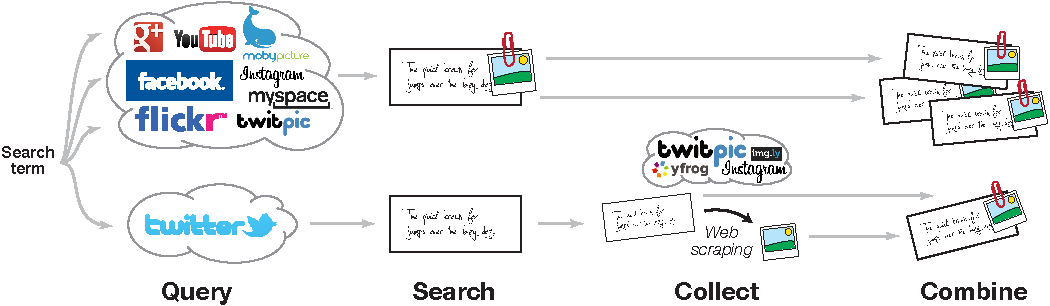
\includegraphics[width=1.0\linewidth]{architecture.pdf}
  \caption{Overview of the media extractor:
    hybrid approach for the media item extraction process using
    a combination of API access and Web scraping}
  \label{fig:architecture}
\end{figure}

%%%  3.3 Media Item Processing  %%%
\subsection{Media Item Processing}
As part of the processing chain, we have limited the number of returned results for each media item extractor to 10 items for videos, and 20 items for images. This explains the tendency to round numbers of results in Table~3, marked with $n+$.

\subsubsection{Machine Translation}
Social networking is happening at a global scale. In consequence, many microposts are authored in languages different from English. In order to still make sense out of those microposts, we apply machine translation to translate non-English microposts to English. We use the Google Translate API\footnote{\url{http://code.google.com/apis/language/translate/v2/getting_started.html}} which, if the source language parameter is left blank, tries first to detect the source language and subsequently translates the micropost to English.

\subsubsection{Part of Speech Tagging}
Our processing chain supports part of speech tagging via an open source JavaScript library called jspos\footnote{\url{http://code.google.com/p/jspos/}},
eventually based on Eric Brill's POS tagger~\cite{brill1992simple}. Part of speech tagging does not yet play an active role in the processing chain. However,
we aim for leveraging the additional data for better micropost analysis in the future.

\subsubsection{Named Entity Disambiguation}
Despite their typical relative brevity, microposts still carry a considerable amount of information. It has been shown how meaning can be added to Facebook microposts through named entity recognition and disambiguation~\cite{AddingMeaningToMicroposts}. We generalize the approach to common microposts,
using the NERD framework~\cite{NERD}.

\subsubsection{Media Item Deduplication}
We try to evaluate the popularity of the media items shared across social networks. This task involves the deduplication of extracted media items.
For images, we use PhotoSweeper\footnote{\url{http://itunes.apple.com/us/app/photosweeper/id463362050?mt=12}}, a commercial image deduplication software and we have manually deduplicated videos. In the future, we aim to perform this task fully automatically but with this work, we have already created a baseline for specific future algorithms tailored to media item deduplication on social networks.

\paragraph{Image Deduplication}
The image duplication software we employed allows for different algorithms to be used. We have applied strict pixel-per-pixel comparison for the detection of \emph{exact} duplicates, i.e. we do \emph{not} count a resized version of an image as exact duplicate. Based on bitmap- or histogram-based similarity comparison methods, we introduce the relatively wide term of \emph{loose} duplicate. Bitmap similarity is based on comparing pixels of size-reduced bitmaps.
For our comparison, we used bitmaps of the size $128 \times 128$ pixels without smoothed edges, which corresponds to the best quality settings in the software.
Histogram similarity is based on comparing histograms of size-reduced bitmaps. This method helps finding similar images despite differences in color saturation and lighting. For both similarity comparison methods, a varying threshold was used. In our experiments, we could not make out a clear winning setting for all events. Rather, even for the same event, only a combination of both similarity comparison methods led to satisfactory results, i.e. to a set of loosely duplicate images that also a human being would have chosen. We would like to highlight, however, that all detected loosely duplicate images were detected algorithmically, which is an important fact for the objective of fully automating the deduplication process.

\paragraph{Video Deduplication}
We have deduplicated the videos in the dataset by first automatically splitting them in shots~\cite{CrowdsourcingEvent}, and then manually comparing the videos shot-wise. We considered \emph{exact} duplicates the videos that shared the same shots and same length. For \emph{loose} duplicates, we manually decided whether the videos showed loosely the same based on human judgment. We do not claim that our results are algorithmically reproducible for loosely similar video detection.

%%%%%%%%%%%%%%%%%%%%%%%%
%%%  4. Experiments  %%%
%%%%%%%%%%%%%%%%%%%%%%%%

\section{Experiments}                                                       \label{sec:experiments}
We run experiments during the period of January 10 to 19, 2012 in which we have selected nine events. For those events, we collected media items and microposts using our media extractor (the dataset as well as the visual summaries are available at \url{http://webmasterapp.net/social/icmr2012/}. We invite the reader to browse the dataset and compile a personal set of loose and exact duplicate media items. YouTube video URLs are signed with a token that expires but they can be accessed by following the \texttt{storyurl} link.

%%%  4.1 Events Considered  %%%
\subsection{Events Considered}
We give a short overview of the nine selected events in order to give the reader the necessary background knowledge.
\newline
\textbf{Assad Speech.} On January 10, 2012, Syrian President Bashar al-Assad delivered a lengthy televised talk strongly defending his government's actions and motivations, despite world pressure on his embattled government for its 10-month crackdown on protesters.
% \footnote{Assad Speech: \url{http://www.cnn.com/2012/01/10/world/meast/syria-unrest/}}
\newline
\textbf{CES Las Vegas.} The International Consumer Electronics Show (CES) is a major technology-related trade show held each January in the Las Vegas Convention Center. Not open to the public, the Consumer Electronics Association-sponsored show typically hosts previews of products and new product announcements.
%\footnote{CES Las Vegas: \url{http://www.cesweb.org/aboutcea.asp}}
\newline
\textbf{Costa Concordia Disaster.} The Costa Concordia is an Italian cruise ship that hit a reef and partially sank on January 13, 2012 off the Italian coast.
The vessel ran aground at Isola del Giglio, Tuscany, resulting in the evacuation of 4,211 people on board.
%\footnote{Coosta Concordia Disaster: \url{http://www.costacruise.com/B2C/USA/Info/concordia_statement.htm}}
\newline
\textbf{Cut the Rope Launch.} On January 10, 2012 during Microsoft's keynote at CES, the HTML5 version of the popular mobile game \textit{Cut the Rope} was announced. This is a sub-event of CES Las Vegas.
%\footnote{Cut the Rope Launch: \url{http://ces.cnet.com/8301-33377_1-57356403/}}
\newline
\textbf{Dixville Notch.} Dixville Notch is an unincorporated village in Dixville township of Coos County, New Hampshire, USA, best known in connection with its longstanding middle-of-the-night vote in the U.S. presidential election. In a tradition that started in the 1960 election, all the eligible voters in Dixville Notch gather at midnight in the ballroom of The Balsams. This year, on January 10, 2012, the voters cast their ballots and the polls officially closed one minute later.
%\footnote{Dixville Notch: \url{http://www.washingtonpost.com/2012/01/09/gIQANslKnP_story.html}}
\newline
\textbf{Free Mobile Launch.} Free Mobile is a French mobile broadband company, part of the Iliad group. On January 10, 2012, a long-awaited mobile phone package for \EUR{19.99} with calls included to 40 countries, texts, multimedia messages and Internet was announced by the Iliad group's Chief Strategy Officer, Xavier Niel.
%\footnote{Free Mobile Launch: \url{http://www.nytimes.com/2012/01/11/technology/iliad-takes-aim-at-top-mobile-operators-in-france.html}}
\newline
\textbf{Blackout SOPA.} The Stop Online Piracy Act (SOPA) is a bill of the United States proposed in 2011 to fight online trafficking in copyrighted intellectual property and counterfeit goods. On January 18, the English Wikipedia, Reddit, and several other Internet companies coordinated a service blackout to protest SOPA and its sister bill, the Protect IP Act. Other companies, including Google, posted links and images in an effort to raise awareness.
%\footnote{Blackout SOPA: \url{http://sopablackout.org/learnmore/}}
\newline
\textbf{Ubuntu TV Launch.} Ubuntu TV by Canonical, based on the user interface Unity, is a variant of the Ubuntu operating system, designed to be a Linux distribution specially adapted for embedded systems in televisions. It was announced by Canonical on January 10, 2012, at CES.
%\footnote{Ubuntu TV: \url{http://www.theverge.com/2012/1/9/2695387/ubuntu-tv-video-hands-on}}
\newline
\textbf{Christian Wulff Case.} Since December 2011, German President Christian Wulff faces controversy over discrepancies in statements about a loan while being governor of Lower Saxony. When the affair settled down, it was revealed that he had applied pressure on Springer Press to delay revelations on the issue until he was back from a visit abroad. When Wulff found out that a tabloid was going to break the story, he left a message on the voice mail of the editor-in-chief in which he threatened to take legal action.
%\footnote{Christian Wulff Case: \url{http://www.spiegel.de/international/germany/0,1518,804631,00.html}}

%%%  4.2 Dataset  %%%
\subsection{Dataset}
Our data set contained 448 images with an average file size of $\sim$0.7MB and 143 videos (Table~2). Some videos are no longer available due to either an account termination or a video takedown by the user (Assad, Dixville). We observed that the process of image deduplication is by no means a solved issue. Content-based image retrieval (CBIR) uses features like color, texture, and shape to search images from large-scale databases. The same technique, however, can also be used for the deduplication of photographs~\cite{Pattabhi:RAICS11}. We used the PhotoSweeper CBIR-based image duplication detection software that allows for manual algorithm and threshold selection to detect duplicates in the dataset (Table~\ref{tab:duplicate-media}).

\begin{table*}[htbp]
  \centering{
  \small{
  \begin{tabular}{|c|c|c|c|c|c|c|c|c|c|c|c|c|c|c|c|c|c|c|}
    \hline
    \multicolumn{1}{|c|}{\textbf{Social}} & \multicolumn{2}{c|}{\textbf{Assad}} & \multicolumn{2}{c|}{\textbf{CES}} &
    \multicolumn{2}{c|}{\textbf{Concordia}} & \multicolumn{2}{c|}{\textbf{Dixville}} & \multicolumn{2}{c|}{\textbf{Free}} &
    \multicolumn{2}{c|}{\textbf{Ropes}} & \multicolumn{2}{c|}{\textbf{SOPA}} & \multicolumn{2}{c|}{\textbf{Ubuntu}} &
    \multicolumn{2}{c|}{\textbf{Wulff}} \\
    \cline{2-19}
    \multicolumn{1}{|c|}{\textbf{Network}} & \textbf{I} & \textbf{V} & \textbf{I} & \textbf{V} & \textbf{I} & \textbf{V} &
    \textbf{I} & \textbf{V} & \textbf{I} & \textbf{V} & \textbf{I} & \textbf{V} & \textbf{I} & \textbf{V} & \textbf{I} &
    \textbf{V} & \textbf{I} & \textbf{V} \\
    \hline
    \textbf{Google+} & 3 & 2 & 5 & 3 & 15 & 1 & 4 & 1 & 6 & 0 & 5 & 1 & 5 & 0 & 6 & 1 & 7 & 0\\
    \textbf{MySpace} & 0 & 0 & 0 & 0 & 10+ & 0 & 9 & 0 & 1 & 0 & 6 & 0 & 0 & 0 & 0 & 0 & 8 & 0\\
    \textbf{Facebook} & 0 & 0 & 0 & 1 & 0 & 1 & 0 & 0 & 0 & 0 & 0 & 0 & 0 & 2 & 0 & 0 & 0 & 0\\
    \textbf{Twitter} & 2 & 0 & 2 & 0 & 3 & 0 & 3 & 0 & 2 & 0 & 4 & 0 & 5 & 0 & 0 & 0 & 2 & 0\\
    \textbf{Instagram} & 0 & 0 & 20+ & 0 & 20+ & 0 & 0 & 0 & 20+ & 0 & 20+ & 0 & 20+ & 0 & 0 & 0 & 2 & 0\\
    \textbf{YouTube} & 0 & 10+ & 0 & 10+ & 0 & 10+ & 0 & 3 & 0 & 10+ & 0 & 10+ & 0 & 10+ & 0 & 10+ & 0 & 10+\\
    \textbf{Flickr} & 10+ & 0 & 10+ & 6 & 10+ & 10+ & 10+ & 10+ & 10+ & 0 & 10+ & 10+ & 10+ & 0 & 10+ & 9 & 10+ & 2\\
    \textbf{MobyPicture} & 0 & 0 & 1 & 0 & 4 & 0 & 0 & 0 & 2 & 0 & 20+ & 0 & 1 & 0 & 2 & 0 & 3 & 0\\
    \textbf{Twitpic} & 0 & 0 & 20+ & 0 & 18 & 0 & 1 & 0 & 20+ & 0 & 20+ & 0 & 19 & 0 & 2 & 0 & 20+ & 0\\
    \hline
    \textbf{Total} & 15 & 12 & 58 & 20 & 80 & 22 & 27 & 14 & 61 & 10 & 85 & 21 & 60 & 12 & 20 & 20 & 52 & 12\\
    \hline
  \end{tabular}
  }
  \label{tab:number-media}
  \caption{Number of images and videos collected for the 9 events (resp. \textbf{Assad Speech}, \textbf{CES Las Vegas}, \textbf{Costa Concordia Disaster}, \textbf{Dixville Notch}, \textbf{Free Mobile Launch}, \textbf{Cut the Rope Launch}, \textbf{Blackout SOPA}, \textbf{Ubuntu TV Launch} and \textbf{Christian Wulff Case}) grouped by social networks}
  }
\end{table*}

For each event, we have manually selected the best settings to limit the number of duplicate misses and false positives. The main problem with the dataset is its diversity. It ranges from entirely sharp screenshots in all sorts of formats (e.g. screenshots of the Google homepage for the Blackout SOPA event), to blurry cell phone images in standard photo formats (e.g. photos of the stage for the Free Mobile Launch event). A common performance tweak to speed up the duplication detection process is to shrink images to quadratic bitmaps. In the context of our dataset, however, this approach is counter productive, as a screenshot of a rectangular IAB $728 \times 90$ ``leaderboard'' banner is treated the same as a standard 3.1 megapixels ($2048 \times 1536$) cell phone photo. In practice, shrinking a wide rectangular banner to a square led to many incorrect results requiring manual deduplication with the Blackout SOPA event.

\begin{table*}[htbp]
  \begin{tabular}{|c|c|c||c|c|}
    \hline
    \textbf{Event} & \textbf{Exact Duplicate I} & \textbf{Loose Duplicate I} & \textbf{Exact Duplicate V} & \textbf{Loose Duplicate V}\\
    \hline
    Assad Speech & 0 image in 0 seq & 2 images in 1 seq & 0 video in 0 seq & 2 videos in 1 seq\\
    CES Las Vegas & 0 image in 0 seq & 9 images in 3 seq & 0 video in 0 seq & 2 videos in 1 seq\\
    Costa Concordia & 0 image in 0 seq & 6 images in 3 seq & 0 video in 0 seq & 0 video in 0 seq\\
    Cut the Rope Launch & 2 images in 1 seq & 15 images in 5 seq & 0 video in 0 seq & 14 videos in 3 seq\\
    Dixville Notch & 2 images in 1 seq & 2 images in 1 seq & 2 videos in 1 seq & 0 video in 0 seq\\
    Free Mobile Launch & 2 images in 1 seq & 16 images in 7 seq & 0 video in 0 seq & 0 video in 0 seq\\
    Blackout SOPA & 0 image in 0 seq & 14 images in 4 seq & 2 videos in 1 seq & 0 video in 0 seq\\
    Ubuntu TV Launch & 0 image in 0 seq & 5 images in 1 seq & 4 videos in 1 seq & 9 videos in 4 seq\\
    Christian Wulff Case & 4 images in 2 seq & 0 image in 0 seq & 0 video in 0 seq & 0 video in 0 seq\\
    \hline
  \end{tabular}
  \label{tab:duplicate-media}
  \caption{Exact and loose duplicate images (I) and videos (V) per event}
\end{table*}

%Some videos are false positives (Cut the rope launch, Dixville, Free mobile, Ubuntu).

%%%  4.3 Ranking Media Items  %%%
\subsection{Ranking Media Items}
Looking at our dataset, it is obvious that the amount of exact duplicate images and videos is largely inferior compared to the amount of loose duplicates. On the one hand, this is owed to applied search operators that exclude re-shared microposts such as Re-Tweets of the same tweet. Hence, the same media item can appear twice in our results only if two users authored different microposts referencing the same media item. On the other hand, it is also owed to our strict definition of exact duplicate which counts resized versions of the same media item as different. We argue that this makes sense as someone had to actively process the media item. A good example is the Blackout SOPA event where the text in the first sequence in \autoref{fig:sequences} is identical while the images have different file sizes, resolutions and paddings. This implies that someone has taken the initial image and applied some post-processing (e.g. cropping) before re-sharing it. A similar example is the second sequence in \autoref{fig:sequences} of the Costa Concordia Disaster where the chimney got cut off.

Long term access to the media items that have been extracted is fragile if only the reference is kept. Users can terminate their accounts on social networks,
delete media items, or change their privacy settings at any time. In addition, social networks can themselves remove media items according to their policies or government order. Hence, in the context of the Assad Speech event, we experienced media items that were quickly no longer available.
%To be on the safe side, only media items where explicitly the media item owner as well as the social network permit storage by third parties should be stored.
%We did not consider legal requirements, however, do note that for potential future exploitation this is indispensable.

By clustering loose duplicate media items in sequences, we aim at boosting diversity in the returned set of media items for a given event: if there are many media items for an event, in the long term we try to only show the most relevant ones from each sequence. This will require a media item ranking formula that will include a combination of different categories of ranking criteria:
\newline
\textbf{Visual Features.} Extracted visual features from media items can help judge their quality. Sharp is better than blurry, higher contrast is better than lower contrast, etc. Interestingly, we observe that videos with less or just one camera shot are more likely produced by amateurs, while videos with more shots are more likely produced by professionals. Depending on the event, one might be preferred over the other.
\newline
\textbf{Low-level Features.} Common low-level features such as resolution, file size, but also the presence of EXIF metadata or geolocation are good quality indicators. Longer videos are better than shorter videos, higher resolution is better than lower resolution, etc.
\newline
\textbf{Social Features.} Media items belonging to the same sequence can have different popularity, either globally across social networks, or on specific social networks. Combining network-specific signals (e.g. number of Re-Tweets on Twitter, Likes on Facebook, +1s on Google+, views on YouTube) and generic signals (e.g. number of comments to a micropost) help to generate a good social popularity indicator. This can also include user diversity by featuring content from different users rather than just content from one user.
\newline
\textbf{Textual Features.} Media items are often surrounded by a textual description in a micropost. Named entity disambiguation can reveal valuable insights which can be further combined with face recognition techniques in order to select media items. Assuming that a user sends a micropost containing a media item about a concert while mentioning the name of a singer. A framework such as NERD can map the singer's name to a Linked Data concept and help searching for known objects such as the singer's face.

\begin{figure*}
\begin{tabular}{p{\textwidth}}
\eventtitle{Blackout SOPA}
\begin{thumbsequence}
		\includegraphics[height=\thumbheight]{sopa/looseduplicate1.jpg}
		\includegraphics[height=\thumbheight]{sopa/looseduplicate2.jpg}
		\includegraphics[height=\thumbheight]{sopa/looseduplicate3.jpg}
		\includegraphics[height=\thumbheight]{sopa/looseduplicate4.jpg}
		\includegraphics[height=\thumbheight]{sopa/looseduplicate5.jpg}
		\includegraphics[height=\thumbheight]{sopa/looseduplicate6.jpg}
	\end{thumbsequence}
	\begin{thumbsequence}
		\includegraphics[height=\thumbheight]{sopa/looseduplicate7.png}
		\includegraphics[height=\thumbheight]{sopa/looseduplicate8.jpg}
	\end{thumbsequence}
	\newstrip
	\begin{thumbsequence}
		\includegraphics[height=\thumbheight]{sopa/looseduplicate9.png}
		\includegraphics[height=\thumbheight]{sopa/looseduplicate10.png}
		\includegraphics[height=\thumbheight]{sopa/looseduplicate11.jpg}
		\includegraphics[height=\thumbheight]{sopa/looseduplicate12.jpg}
	\end{thumbsequence}
	\begin{thumbsequence}
		\setlength\fboxsep{0pt}
		\setlength\fboxrule{0.1mm}
		\fbox{\includegraphics[height=\thumbheight]{sopa/looseduplicate13.png}}
		\fbox{\includegraphics[height=\thumbheight]{sopa/looseduplicate14.jpg}}
\end{thumbsequence}
\end{tabular}

\vspace{.5em}
	
\begin{tabular}{p{\textwidth}}
\eventtitle{Christian Wulff Case}
	\begin{thumbsequence}
		\doublebox{\includegraphics[height=\thumbheight]{wulff/exactduplicate1.jpg}}
		\doublebox{\includegraphics[height=\thumbheight]{wulff/exactduplicate2.jpg}}
	\end{thumbsequence}
	\begin{thumbsequence}
		\doublebox{\includegraphics[height=\thumbheight]{wulff/exactduplicate3.jpg}}
		\doublebox{\includegraphics[height=\thumbheight]{wulff/exactduplicate4.jpg}}
	\end{thumbsequence}
\end{tabular}

\vspace{.5em}

\begin{tabular}{p{.5\textwidth}p{.5\textwidth}}
\eventtitle{Dixville Notch}
	\begin{thumbsequence}
		\doublebox{\includegraphics[height=\thumbheight]{dixville/exactduplicate1.jpg}}
		\doublebox{\includegraphics[height=\thumbheight]{dixville/exactduplicate2.jpg}}
	\end{thumbsequence}
	\begin{thumbsequence}
		\includegraphics[height=\thumbheight]{dixville/looseduplicate1.jpg}
		\includegraphics[height=\thumbheight]{dixville/looseduplicate2.jpg}
	\end{thumbsequence}
	&
\vspace{-3pt}
\eventtitle{Assad Speech}
	\begin{thumbsequence}
		\includegraphics[height=\thumbheight]{assad/looseduplicate1.jpg}
		\includegraphics[height=\thumbheight]{assad/looseduplicate2.jpg}
	\end{thumbsequence}
\end{tabular}

\vspace{.5em}

\begin{tabular}{p{\textwidth}}
\eventtitle{Free Mobile Launch}
	\begin{thumbsequence}
		\doublebox{\includegraphics[height=\thumbheight]{free/exactduplicate1.jpg}}
		\doublebox{\includegraphics[height=\thumbheight]{free/exactduplicate2.jpg}}
	\end{thumbsequence}
	\begin{thumbsequence}
		\includegraphics[height=\thumbheight]{free/looseduplicate1.png}
		\includegraphics[height=\thumbheight]{free/looseduplicate2.png}
	\end{thumbsequence}
	\begin{thumbsequence}
		\includegraphics[height=\thumbheight]{free/looseduplicate7.jpg}
		\includegraphics[height=\thumbheight]{free/looseduplicate8.jpg}
	\end{thumbsequence}
	\\[4pt]
	\begin{thumbsequence}
		\includegraphics[height=\thumbheight]{free/looseduplicate15.jpg}
		\includegraphics[height=\thumbheight]{free/looseduplicate16.png}
	\end{thumbsequence}
	\begin{thumbsequence}
		\includegraphics[height=\thumbheight]{free/looseduplicate9.jpg}
		\includegraphics[height=\thumbheight]{free/looseduplicate10.jpg}
		\includegraphics[height=\thumbheight]{free/looseduplicate11.jpg}
	\end{thumbsequence}
	\begin{thumbsequence}
		\includegraphics[height=\thumbheight]{free/looseduplicate3.jpg}
		\includegraphics[height=\thumbheight]{free/looseduplicate4.jpg}
	\end{thumbsequence}
	\newstrip
	\begin{thumbsequence}
		\includegraphics[height=\thumbheight]{free/looseduplicate12.jpg}
		\includegraphics[height=\thumbheight]{free/looseduplicate13.jpg}
		\includegraphics[height=\thumbheight]{free/looseduplicate14.jpg}
	\end{thumbsequence}
	\begin{thumbsequence}
		\includegraphics[height=\thumbheight]{free/looseduplicate5.jpg}
		\includegraphics[height=\thumbheight]{free/looseduplicate6.jpg}
	\end{thumbsequence}
\end{tabular}

\vspace{.5em}

\begin{tabular}{p{\textwidth}}
\eventtitle{Costa Concordia Disaster}
	\begin{thumbsequence}
		\includegraphics[height=\thumbheight]{concordia/looseduplicate1.jpg}
		\includegraphics[height=\thumbheight]{concordia/looseduplicate2.jpg}
	\end{thumbsequence}
	\begin{thumbsequence}
		\includegraphics[height=\thumbheight]{concordia/looseduplicate3.jpg}
		\includegraphics[height=\thumbheight]{concordia/looseduplicate4.jpg}
	\end{thumbsequence}
	\begin{thumbsequence}
		\includegraphics[height=\thumbheight]{concordia/looseduplicate5.jpg}
		\includegraphics[height=\thumbheight]{concordia/looseduplicate6.jpg}
	\end{thumbsequence}
\end{tabular}

\vspace{.5em}

\begin{tabular}{p{\textwidth}}
\eventtitle{CES Las Vegas}
	\begin{thumbsequence}
		\includegraphics[height=\thumbheight]{ces/looseduplicate1.jpg}
		\includegraphics[height=\thumbheight]{ces/looseduplicate2.jpg}
		\includegraphics[height=\thumbheight]{ces/looseduplicate3.jpg}
		\includegraphics[height=\thumbheight]{ces/looseduplicate4.jpg}
		\includegraphics[height=\thumbheight]{ces/looseduplicate5.jpg}
	\end{thumbsequence}
	\begin{thumbsequence}
		\includegraphics[height=\thumbheight]{ces/looseduplicate6.jpg}
		\includegraphics[height=\thumbheight]{ces/looseduplicate7.jpg}
	\end{thumbsequence}
	\begin{thumbsequence}
		\includegraphics[height=\thumbheight]{ces/looseduplicate8.jpg}
		\includegraphics[height=\thumbheight]{ces/looseduplicate9.jpg}
	\end{thumbsequence}
\end{tabular}

\vspace{.5em}

\begin{tabular}{p{.5\textwidth}p{.5\textwidth}}
	\eventtitle{Cut the Rope Launch}
	\begin{thumbsequence}
		\doublebox{\includegraphics[height=\thumbheight]{ropes/exactduplicate1.jpg}}
		\doublebox{\includegraphics[height=\thumbheight]{ropes/exactduplicate2.jpg}}
	\end{thumbsequence}
	\begin{thumbsequence}
		\includegraphics[height=\thumbheight]{ropes/looseduplicate5.jpg}
		\includegraphics[height=\thumbheight]{ropes/looseduplicate6.jpg}
		\includegraphics[height=\thumbheight]{ropes/looseduplicate7.jpg}
		\includegraphics[height=\thumbheight]{ropes/looseduplicate8.jpg}
		\includegraphics[height=\thumbheight]{ropes/looseduplicate9.jpg}
	\end{thumbsequence}
	\newline\vspace{-.5em}\newline
	\begin{thumbsequence}
		\includegraphics[height=\thumbheight]{ropes/looseduplicate12.jpg}
		\includegraphics[height=\thumbheight]{ropes/looseduplicate13.jpg}
	\end{thumbsequence}
	\begin{thumbsequence}
		\includegraphics[height=\thumbheight]{ropes/looseduplicate14.jpg}
		\includegraphics[height=\thumbheight]{ropes/looseduplicate15.jpg}
	\end{thumbsequence}
	\begin{thumbsequence}
		\includegraphics[height=\thumbheight]{ropes/looseduplicate10.jpg}
		\includegraphics[height=\thumbheight]{ropes/looseduplicate11.jpg}
	\end{thumbsequence}
	\newstrip
	\begin{thumbsequence}
		\includegraphics[height=\thumbheight]{ropes/looseduplicate1.jpg}
		\includegraphics[height=\thumbheight]{ropes/looseduplicate2.jpg}
		\includegraphics[height=\thumbheight]{ropes/looseduplicate3.png}
		\includegraphics[height=\thumbheight]{ropes/looseduplicate4.png}
	\end{thumbsequence}
	&
\eventtitle{Ubuntu TV launch}
	\begin{thumbsequence}
		\includegraphics[height=\thumbheight]{ubuntu/looseduplicate1.jpg}
		\includegraphics[height=\thumbheight]{ubuntu/looseduplicate2.jpg}
		\newstrip
		\includegraphics[height=\thumbheight]{ubuntu/looseduplicate3.jpg}
		\includegraphics[height=\thumbheight]{ubuntu/looseduplicate4.jpg}
		\newstrip
		\includegraphics[height=\thumbheight]{ubuntu/looseduplicate5.png}
	\end{thumbsequence}
\end{tabular}
\caption{Results of the image deduplication (exact and loose duplicate) for the 9 selected events}
\label{fig:sequences}
\end{figure*}

%%%  4.4 Generating Media Galleries  %%%
\subsection{Generating Media Galleries}
Once the media items are ranked, it is possible to generate media galleries and build visual summaries. Popular media items can be displayed bigger, longer, or with a special decoration like a thicker border in comparison to less popular media items. For videos, the audio part poses a challenge. In our experiments, we observe that intermixing the audio of all videos of an event often generates a very characteristic ``noise cloud''. A good example is the Assad Speech event, where a mix of Arabic voices blends nicely with the speech of a US politician. A different example is the CES Las Vegas event, where the atmosphere of a big exposition with music, announcements, and technical analysis becomes alive.

%%%%%%%%%%%%%%%%%%%%%%%%%
%%%  5. Related Work  %%%
%%%%%%%%%%%%%%%%%%%%%%%%%

\section{Related Work}                                                      \label{sec:related-work}
% Separate related work in fields:
% - media item collection from social networks
% - event summarization
% Highlight what Twitter is doing (most popular image/video)
% Google news top stories
% Automatic gallery creation

A~first category of related work includes research that aims to collect, align, and organize media for trends or events.
Liu \emph{et al.} combine semantic inferencing and visual analysis to automatically find media to illustrate events~\cite{Liu:ICMR11}.
They interlink large datasets of event metadata and media with the Linking Open Data Cloud~\cite{LODcloud}.
Approaches for alignment use visual, temporal, and spacial similarity measures to map multiple photo streams of the same events~\cite{Yang2011}.
Other ways to collect and order media from social networks use user-driven metadata such as geospatial information~\cite{Crandall}.

Another relevant work area is duplicate and near-duplicate media detection. Work on ordinal measures for image correspondence started in the last decade of the 20\superscript{th}~century~\cite{Bhat}. Recently, Chum \emph{et al.} have proposed a near-duplicate image detection method using MinHash and tf--idf weighting~\cite{Chum}. A~method for both images and video has been proposed by Yang \emph{et al.}~\cite{Yang}. Specialized methods for video exist as well~\cite{Min, Wu}, an excellent survey of which has been conducted by Lian \emph{et al.}~\cite{Lian}.

When unique media items have been collected, the remaining task is to summarize events by selecting the most relevant media fragments. Fabro and B\"osz\"orm\'enyi~\cite{Fabro:MMM12} detail the summarization and presentation of events from content retrieved from social media. Nowadays, many domain-specific methods already exhibit good accuracy, for example in the sports domain~\cite{Li1,Li2}. However, the challenge in this field is to find methods that are content-agnostic. Methods that exploit semantic information~(\emph{e.g.} \cite{Chen}) will likely provide high-quality results in the future, but today's most relevant summaries are produced by user interaction~\cite{Olsen}.

%%%%%%%%%%%%%%%%%%%%%%%%%%%%%%%%%%%%%%%
%%%  6. Conclusion and Future Work  %%%
%%%%%%%%%%%%%%%%%%%%%%%%%%%%%%%%%%%%%%%

\section{Conclusion and Future Work}                                        \label{sec:conclusion}
In this section, we presented a generic media extractor for gathering media items shared on social networks and illustrating known events. We proposed a common schema for aligning the search results of these platforms. We further described a full processing chain of the media items that includes machine translation, POS tagging, named entity disambiguation and media item deduplication. We show how media items can be ranked in order to generate visual summaries that convey the feeling of the wisdom of the crowd for a known event.

Our implementation for extracting visual media and associated textual messages covers already most of the Western social networks. We plan to support more social networks used in other parts of the world while improving the Web scrapers in order to significantly improve the quantity and diversity of media and messages shared for an event. Multimedia analysis techniques should be better integrated in the processing chain as this will create a multi-modal environment where different factors are used to organize social content. Hence, content deduplication and visual quality metrics (sharpness, contrast\ldots) can be used to rank the media items. Furthermore, the identification of the original content can allow users to choose a balance between popularity (favor omnipresent content) and originality (promote rare content).

Context-aware multimedia analysis will likely bring a new range of parameters into play since many media items contain a message that is complementary to the text. For example, facial detection~\cite{ViolaJones} and eventually recognition~\cite{Wright} can signify the presence of specific people in a media fragment.
As visual recognition systems grow more powerful, more objects will eventually be recognizable by machines~\cite{Serre}, which would allow generating \emph{visual hashtags} that describe the content \emph{inside} of the media item. Extracted features in all three categories~(\emph{textual} -- from the micropost, \emph{visual} -- from the media item, and \emph{social} -- from the social network in the form of ReTweets, Likes, +1s\ldots) can also serve as ranking criteria, be it in isolation, or in combination by introducing a ranking formula. As a result, this would also positively influence the diversity of automated summarizations.

Nonetheless, it remains important to view the media and the associated text as a whole, since the text could convey a sentiment about or an explanation of the visual data. Using named entity recognition~\cite{NERD,AddingMeaningToMicroposts}, the important semantic elements in the message text can be identified. The content of the message could subsequently be used to narrow down the search space for visual factors enabling cross-fertilization between the textual and visual analysis, which results in effective context-aware analysis possibilities~\cite{verborgh_mtap_2011}.

\section*{Chapter Notes}
This chapter is partly based on the following publications:
\todo{Add publications}

% this file is called up by thesis.tex
% content in this file will be fed into the main document

%: ----------------------- introduction file header -----------------------
\chapter{Media Item Deduplication}

% the code below specifies where the figures are stored
\ifpdf
    \graphicspath{{6_media_item_deduplication/figures/PNG/}{6_media_item_deduplication/figures/PDF/}{6_media_item_deduplication/figures/}}
\else
    \graphicspath{{6_media_item_deduplication/figures/EPS/}{6_media_item_deduplication/figures/}}
\fi

% ----------------------------------------------------------------------
%: ------------------------------- content ----------------------------- 
% ----------------------------------------------------------------------

\section{Image Deduplication}

\section{Video Deduplication}

\section{State of the Art}

\section{Evaluation}

\section{Conclusion}

% this file is called up by thesis.tex
% content in this file will be fed into the main document

%: ----------------------- introduction file header -----------------------
\chapter{Media Item Ranking}

% the code below specifies where the figures are stored
\ifpdf
    \graphicspath{{7_media_item_ranking/figures/PNG/}{7_media_item_ranking/figures/PDF/}{7_media_item_ranking/figures/}}
\else
    \graphicspath{{7_media_item_ranking/figures/EPS/}{7_media_item_ranking/figures/}}
\fi

% ----------------------------------------------------------------------
%: ------------------------------- content ----------------------------- 
% ----------------------------------------------------------------------

\section{Ranking Criteria}

\section{Ranking Formula}

\section{State of the Art}

\section{Evaluation}

\section{Conclusion}
\chapter{Media Item Compilation}
\label{cha:media-item-compilation}

% the code below specifies where the figures are stored
\ifpdf
    \graphicspath{{8_media_item_compilation/figures/PNG/}{8_media_item_compilation/figures/PDF/}{8_media_item_compilation/figures/}}
\else
    \graphicspath{{8_media_item_compilation/figures/EPS/}{8_media_item_compilation/figures/}}
\fi

\section{Introduction}

In this chapter, we present and define aesthetic principles
for the automatic generation of media galleries
based on media items retrieved from social networks
that---after a~ranking and pruning step---can serve to authentically
summarize events and their atmosphere from a~visual
and an audial standpoint.
Mobile devices such as smartphones, together with social networks,
enable people to create, share, and consume media items
like videos or photos.
They accompany their owners almost everywhere
and are thus omnipresent at all sorts of events.
Given a~stable network connection, event-related media items
and microposts are published on social networks
during events and afterwards.
Ranked media items stemming from multiple social networks
can serve to create authentic media galleries
that illustrate events and their atmosphere.
A~key feature for this task is the semantic enrichment
of media items and associated microposts
and the extraction of \textbf{visual}, \textbf{audial},
\textbf{textual}, and \textbf{social} features.
Based on this set of features,
additional \textbf{aesthetic} features
can be defined and exploited to obtain appealing
and harmonic media galleries.

\begin{figure}[htb]
  \centering
  \includegraphics[trim=20mm 40mm 20mm 10mm, clip, width=0.75\columnwidth]{media-gallery.pdf}
  \caption{Schematic media gallery with four photos and two videos.}
  \label{fig:media-gallery}
\end{figure}

\section{Related Work}
While enormous efforts have been made to extract those features
from media items and microposts on social networks in \emph{isolation},
to the best knowledge of the authors, remarkably less initiatives 
concern the extraction and the application
of all those features \emph{in combination}
for \emph{all} types of media items, including microposts.
In~\cite{Photo2011}, Sandhaus \emph{et al.}\ consider visual and
aesthetic features for the automatic creation of photo books.
Obrador \emph{et al.}\ use visual and aesthetic features
for a~category-based approach to automatically assess
the aesthetic appeal of photographs~\cite{Photo2012}.
In~\cite{Playlist2006}, Knees \emph{et al.}\ use audial and textual
features for the automatic generation of music playlists.
Choudhury \emph{et al.}\ show in\cite{Sports2011} how social and textual
features can be used to achieve precise detection results 
of named entities and significant events in sports-related microposts.
In~\cite{YouTube2010}, Davidson \emph{et al.}\ show how visual,
textual, and social features can be used for personalized video recommendations.
A service called Storify~\cite{Storify2011} lets users manually combine
microposts, photos, videos, and other elements onto one page for the purpose
of storytelling or summarizing an event,
and share stories permanently on the Web.
Finally, social networks present photos and videos
often in grid-like galleries\footnote{\url{http://twitpic.com/904yka/full}}, sometimes scaled
based on the amount of comments.
When unique media items have been collected, the remaining task is to summarize events by selecting the most relevant media fragments. Fabro and B\"osz\"orm\'enyi~\cite{Fabro:MMM12} detail the summarization and presentation of events from content retrieved from social media. Nowadays, many domain-specific methods already exhibit good accuracy, for example in the sports domain~\cite{Li1,Li2}. However, the challenge in this field is to find methods that are content-agnostic. Methods that exploit semantic information~(\emph{e.g.}~\cite{Chen}) will likely provide high-quality results in the future, but today's most relevant summaries are produced by user interaction~\cite{Olsen}.

\section{Media Gallery Aesthetics}

\noindent \textbf{Definition}
A media gallery in our context is a~compilation of photos or videos
retrieved from social networks that are related to a~given event.
Given a~set $M = \{m_1,..., m_n\}$ of media items related to a~certain event,
and given a~ranking formula $f$,
the subset $M^\prime \subset M$
is the result after the application of $f$ to $M$: $f(M)=M^\prime$.
Each media item $m_i$ can either be an instance of video or photo.
For each point $t_x$ on a~timeline $T$, the state of the media gallery
at $t_x$ is defined for each media item $m_i$
as a~set $S_x$ of $n$ tuples $s_{x,i}$, where
$s_{x,i}=\langle \mathit{left}$, $\mathit{top}$, $\mathit{width}$, $\mathit{height}$,
$\mathit{alpha}$, $\mathit{z\mbox{-}index}$, $\mathit{animation}$,
$\mathit{start}$, $\mathit{playing}$, $\mathit{volume} \rangle$.
The first 6~properties are defined as in CSS, the $\mathit{animation}$ property
allows for the definition of CSS transitions
and transformations as defined in~\cite{CSSTransitions2009,CSSTransforms2012},
the $\mathit{start}$ property defines the start time in a~video.
A schematic media gallery at $t_x$ can be seen in \autoref{fig:media-gallery}.

\noindent \textbf{Audial aesthetics}
We recall the purpose of our media galleries:
to illustrate an event and its atmosphere.
Audial aesthetics thus consist of aspects like volume level normalization,
avoiding multiple videos playing music in parallel, smooth transitions, \emph{etc}.
We remark that through selective mixing of audio tracks
of event-related videos, ``noise clouds'' very characteristic
for the event atmosphere can be observed.

\noindent \textbf{Visual aesthetics}
Visual aesthetics are determined by the composition, \emph{i.e.},
the relation of photos to videos \emph{globally}, \emph{per coherent scene},
and per \emph{point in time}.
In order not to overcharge the perceptive capacity
of viewers, the number of visible (moving) media items
at a~time should be limited.
Depending on the event, a~consistent or a~contrasty overall
appearance of items may be desired, also for transitions.

\begin{figure}[htb]
  \centering
  \includegraphics[width=0.75\linewidth]{inaug2013}
  \caption[Automatically generated media gallery for Obama's inauguration 2013]{Automatically generated media gallery in the context of President Barack Obama's inauguration 2013}
  \label{fig:inaug2013}
\end{figure}

\begin{figure}[htb]
  \centering
  \includegraphics[width=0.75\linewidth]{30u30}
  \caption[Automatically generated media gallery in the context of the 30u30 event]{Automatically generated media gallery in the context of the 30u30 event, a~young professionals initiative where 30 persons younger than 30 gathered (\url{http://prreport.de/home/aktuell/article/6390-30-junge-aufsteiger-in-der-kommunikationsbranche/},
  accessed Janaury 22, 2013)}
  \label{fig:30u30}
\end{figure}


\section{Conclusion}
We have introduced media item ranking criteria, and
aesthetic audial and visual principles for media galleries.
In the coming months, we will apply those principles
to a~large collection of media items related to events,
and, via multivariate tests, measure user engagement
for different feature configurations.

\section*{Chapter Notes}
This chapter is partly based on the following publications:
\todo{Add publications}

% this file is called up by thesis.tex
% content in this file will be fed into the main document

%: ----------------------- introduction file header -----------------------
\chapter{Future Work}

% the code below specifies where the figures are stored
\ifpdf
    \graphicspath{{9_future_work/figures/PNG/}{9_future_work/figures/PDF/}{9_future_work/figures/}}
\else
    \graphicspath{{9_future_work/figures/EPS/}{9_future_work/figures/}}
\fi

% ----------------------------------------------------------------------
%: ------------------------------- content ----------------------------- 
% ----------------------------------------------------------------------

\section{Contributions}

\section{Research Directions}






% this file is called up by thesis.tex
% content in this file will be fed into the main document

%: ----------------------- introduction file header -----------------------
\chapter{Conclusion}

% the code below specifies where the figures are stored
\ifpdf
    \graphicspath{{1_introduction/figures/PNG/}{1_introduction/figures/PDF/}{1_introduction/figures/}}
\else
    \graphicspath{{1_introduction/figures/EPS/}{1_introduction/figures/}}
\fi

% ----------------------------------------------------------------------
%: ------------------------------- content ----------------------------- 
% ----------------------------------------------------------------------

\section{Summary}

\section{Retrospect}


% --------------------------------------------------------------
%:                  BACK MATTER: appendices, refs,..
% --------------------------------------------------------------

% the back matter: appendix and references close the thesis

%: Appendices
% this file is called up by thesis.tex
% content in this file will be fed into the main document

%: ----------------------- introduction file header -----------------------

\chapter{Appendices}
\appendix

% the code below specifies where the figures are stored
\ifpdf
    \graphicspath{{backmatter/figures/PNG/}{backmatter/figures/PDF/}{backmatter/figures/}}
\else
    \graphicspath{{backmatter/figures/EPS/}{backmatter/figures/}}
\fi

% ----------------------------------------------------------------------
%: ------------------------------- content ----------------------------- 
% ----------------------------------------------------------------------

\section*{Curriculum Vit{\ae}}

\todo{Add resume}

\section*{Publications}

\todo{Add publications}

%: ----------------------- bibliography ------------------------

% The section below defines how references are listed and formatted
% The default below is 2 columns, small font, complete author names.
% Entries are also linked back to the page number in the text and to external URL if provided in the BibTex file.

% PhDbiblio-url2 = names small caps, title bold & hyperlinked, link to page 
\begin{multicols}{2} % \begin{multicols}{ # columns}[ header text][ space]
\begin{tiny} % tiny(5) < scriptsize(7) < footnotesize(8) < small (9)

\bibliographystyle{Latex/Classes/PhDbiblio-url2} % Title is link if provided
% --------------------------------------------------------------
% Various bibliography styles exit. Replace above style as desired.

% in-text refs: (1) (1; 2)
% ref list: alphabetical; author(s) in small caps; initials last name; page(s)
%\bibliographystyle{Latex/Classes/PhDbiblio-case} % title forced lower case
%\bibliographystyle{Latex/Classes/PhDbiblio-bold} % title as in bibtex but bold
%\bibliographystyle{Latex/Classes/PhDbiblio-url} % bold + www link if provided

%\bibliographystyle{Latex/Classes/jmb} % calls style file jmb.bst
% in-text refs: author (year) without brackets
% ref list: alphabetical; author(s) in normal font; last name, initials; page(s)

%\bibliographystyle{plainnat} % calls style file plainnat.bst
% in-text refs: author (year) without brackets
% (this works with package natbib)

\renewcommand{\bibname}{References} % changes the header; default: Bibliography

\bibliography{backmatter/references} % adjust this to fit your BibTex file

\end{tiny}
\end{multicols}

% --------------------------------------------------------------

%: Declaration of originality

% Thesis statement of originality -------------------------------------

% Depending on the regulations of your faculty you may need a declaration like the one below. This specific one is from the medical faculty of the university of Dresden.

\begin{declaration}        %this creates the heading for the declaration page

I herewith declare that I have produced this document without the prohibited assistance of third parties and without making use of aids other than those specified; notions taken over directly or indirectly from other sources have been identified as such. This document has not previously been presented in identical or similar form to any other examination board.

The thesis work was conducted from February 2010 to July 2013 under the supervision of Joaquim Gabarró Vallés (Universitat Politècnica de Catalunya, Barcelona, Spain) and Michael Hausenblas (Digital Enterprise Research Institute, Galway, Ireland and MapR Technologies, San Jose, CA, USA).

\vspace{10mm}

Barcelona, in February 2014

\end{declaration}

\cleardoublepage

% ----------------------------------------------------------------------

\end{document}
